\chapter{Active Set pour la résolution de problèmes de contact en milieu déformable}\label{chap:active-set-deformable}


\newcommand{\blambda}{\mbox{\boldmath{$\lambda$}}}
\newcommand{\bLambda}{\mbox{\boldmath{$\Lambda$}}}
\newcommand{\bmu}{\mbox{\boldmath{$\mu$}}}
\newcommand{\btheta}{\mbox{\boldmath{$\theta$}}}
\newcommand{\bPi}{\mbox{\boldmath{$\Pi$}}}
\newcommand{\bW}{\mbox{\boldmath{$W$}}}
\newcommand{\bM}{\mbox{\boldmath{$M$}}}
\newcommand{\bN}{\mbox{\boldmath{$N$}}}
\newcommand{\bV}{\mbox{\boldmath{$V$}}}
\newcommand{\bP}{\mbox{\boldmath{$P$}}}
\newcommand{\bS}{\mbox{\boldmath{$S$}}}
\newcommand{\bQ}{\mbox{\boldmath{$Q$}}}
\newcommand{\be}{\mbox{\boldmath{$e$}}}
\newcommand{\bu}{\mbox{\boldmath{$u$}}}
\newcommand{\bU}{\mbox{\boldmath{$U$}}}
\newcommand{\Mb}{\mbox{\boldmath{$M$}}}
\newcommand{\bL}{\mbox{\boldmath{$L$}}}
\newcommand{\bv}{\mbox{\boldmath{$v$}}}
\newcommand{\bn}{\mbox{\boldmath{$n$}}}
\newcommand{\br}{\mbox{\boldmath{$r$}}}
\newcommand{\bw}{\mbox{\boldmath{$w$}}}
\newcommand{\bvs}{\mbox{\boldmath{\footnotesize$v$}}}
\newcommand{\bx}{\mbox{\boldmath{$x$}}}
\newcommand{\bxi}{\mbox{\boldmath{$\xi$}}}
\newcommand{\by}{\mbox{\boldmath{$y$}}}
\newcommand{\bz}{\mbox{\boldmath{$z$}}}
\newcommand{\bF}{\mbox{\boldmath{$F$}}}
\newcommand{\bI}{\mbox{\boldmath{$I$}}}
\newcommand{\bg}{\mbox{\boldmath{$g$}}}
\newcommand{\fb}{\mbox{\boldmath{$f$}}}
\newcommand{\bh}{\mbox{\boldmath{$h$}}}
\newcommand{\bsigma}{\mbox{\boldmath{$\sigma$}}}
\newcommand{\btau}{\mbox{\boldmath{$\tau$}}}
\newcommand{\bvarphi}{\mbox{\boldmath{$\varphi$}}}
\newcommand{\bvarepsilon}{\mbox{\boldmath{$\varepsilon$}}}
\newcommand{\bnu}{\mbox{\boldmath{$\nu$}}}
\newcommand{\beeta}{\mbox{\boldmath{$\eta$}}}
\newcommand{\bzeta}{\mbox{\boldmath{$\zeta$}}}
\newcommand{\bbeta}{\mbox{\boldmath{$\beta$}}}
\newcommand{\bzero}{\mbox{\boldmath{$0$}}}
\newcommand{\bgamma}{\mbox{\boldmath{$\gamma$}}}
\newcommand{\bpsi}{\mbox{\boldmath{$\psi$}}}
\newcommand{\bphi}{\mbox{\boldmath{$\phi$}}}
\newcommand{\T}{\mathcal{T}}
\newcommand{\cG}{\mbox{{${\cal G}$}}}
\newcommand{\RR}{\mathbb{R}}
\newcommand{\PP}{\mathcal{P}}
\newcommand{\btu}{\tilde{\mbox{\boldmath{$u$}}}}
\newcommand{\dual}[2]{\langle #1 \rangle_{#2^*\times#2}}

\newcommand{\cP}{\mbox{{${\cal P}$}}}



%\newtheorem{theorem}{Theorem}[section]
%\newtheorem{lemma}[theorem]{Lemma}
\newtheorem{corollary}[theorem]{Corollary}
%\newtheorem{definition}[theorem]{Definition}
\newtheorem{proposition}[theorem]{Proposition}

\numberwithin{equation}{section}

\vspace{1cm}


\textit{Dans ce deuxième chapitre, plusieurs méthodes de type Active Set basées sur un schéma itératif semi-régulier de Newton sont fournies à travers des problèmes classiques qui se posent en mécanique du contact en milieu déformable, à savoir des problèmes de contact unilatéral sans frottement, bilatéral avec frottement de Tresca et unilatéral avec frottement de Coulomb en petites et grandes déformations. L'objectif ici, au delà de proposer une méthode numérique de résolution de ces problèmes, est de rappeler que ces méthodes ont été introduites initialement en milieu déformable, notamment dans les travaux de Abide, Barboteu et Danan \cite{abide2016analysis}, complétés par ceux de Abide, Barboteu et Cherkaoui \cite{abide2021inexact} pour la résolution de problèmes de contact élastodynamique avec frottement.}

\vspace{1cm}

\minitoc

\newpage

\section*{Introduction}

Les problèmes de contact avec frottement restent encore de nos jours un sujet d'étude important pour l'analyse mathématique et numérique. Dans la littérature, de nombreuses références proposent différentes approches pour les conditions de contact usuelles (cf \cite{alart1991mixed}, \cite{chabrand1998various}, \cite{chouly2017overview}, \cite{khenous2006hybrid}, \cite{lebon2003contact}, \cite{laursen2013computational}, \cite{raous1988numerical}, \cite{sofonea2012mathematical}, \cite{wriggers2004computational}). Pour gérer les non-linéarités dues aux conditions de contact avec frottement, plusieurs méthodes ont été testées avec succès, à savoir la méthode de pénalisation (cf \cite{kikuchi1988contact}, \cite{oden1982interior}) qui consiste à approcher les conditions d'origine par des conditions plus simples, le quasi-Lagrangien augmenté \cite{alart1991mixed}, la méthode bi-potentiel (cf \cite{de1991new}, \cite{dumont2013enhanced}), la méthode du gradient conjugué (cf \cite{laursen2013computational}, \cite{wriggers2004computational}), la méthode Uzawa (cf \cite{raous1988numerical}, \cite{joli2008uzawa}) et plus récemment, la méthode de Nitsche (cf \cite{chouly2014adaptation}, \cite{chouly2015nitsche}, \cite{chouly2017overview}). Exprimées en termes de  conditions de contact unilatéral (conditions de Signorini) et de frottement de Coulomb, celles-ci conduisent à un problème mathématique non-linéaire et non-régulier. Par conséquent, les équations résultant des problèmes de contact avec frottement semblent être difficiles à résoudre aussi bien mathématiquement que numériquement. Dans ce but, Alart et Curnier, ont proposé dans \cite{alart1991mixed}, une formulation de type quasi-Lagrangien augmenté combinée à une méthode de Newton généralisée pour résoudre ces équations non-différenciables et non-linéaires.
De même, De Saxcé et Feng ont proposé dans \cite{de1991new} une énergie dite bi-potentielle pour prendre en compte le contact avec frottement. Le bi-potentiel, qui n'est pas globalement convexe, est basé sur la théorie du matériau standard implicite et il est minimisé généralement en utilisant une méthode de gradient. La méthode de Nitsche consiste à écrire les conditions de contact directement dans la formulation variationnelle, conduisant à une méthode des éléments finis simple et à un problème discrétisé non-linéaire.\\

Les méthodes Primal-Dual Active Set (PDAS) apparaissent comme l'une des méthodes les plus pertinentes pour résoudre les problèmes de contact avec frottement (cf \cite{hintermuller2002primal}, \cite{hueber2008primal},\cite{hueber2005primal}). Ces méthodes sont basées sur le principe suivant: les conditions de contact et de frottement sont reformulées en termes de fonctions de complémentarités non-linéaires dont la solution est fournie par la méthode itérative semi-régulière de Newton \cite{hintermuller2002primal, hintermuller2003semismooth}. En pratique, le contact avec les conditions de frottement de Coulomb peut être formulé sous forme d'un problème de point fixe lié à un problème de quasi-optimisation. D'un point de vue purement algorithmique, le but principal de ces méthodes est de séparer les noeuds potentiellement en contact en deux sous-ensembles (actifs et inactifs) et de trouver le sous-ensemble correct de tous les noeuds effectivement en contact actifs (sous-ensemble $\cal A$), par opposition à ceux qui sont inactifs (sous-ensemble $\cal I$). En pratique, les méthodes PDAS ne nécessitent pas l'utilisation des multiplicateurs de Lagrange. En fait, les conditions aux limites sur les sous-ensembles $\cal A$ et $\cal I$ sont directement imposées grâce à une méthode semi-régulière (semi-smooth) de Newton, et par conséquent, leur mise en oeuvre pourrait être réalisée sans grand effort. Certains travaux ont été consacrés à l'étude de l'efficacité des méthodes PDAS, ainsi qu'à la résolution de problèmes de contact multicorps non-linéaires pour l'élasticité linéaire (cf \cite{hueber2008primal}, \cite{hueber2005primal}), ainsi qu'à la résolution de problèmes d'élasticité linéaire avec des conditions aux limites unilatérales (cf \cite{hintermuller2002primal},\cite{hintermuller2003semismooth}).\\ 

Dans ce chapitre, nous proposons une méthode PDAS innovante, rapide et efficace pour résoudre un problème hyper-élastodynamique avec contact unilatéral et frottement de Coulomb. Dans un premier temps, l'idée principale de ce chapitre est de présenter en détail la méthode PDAS pour différents cas de contact frottant sur une fondation rigide. Après avoir proposé une méthode PDAS pour le contact unilatéral et pour le contact bilatéral avec frottement de Tresca, nous étendons les résultats obtenus au cas unilatéral avec la loi de frottement de Coulomb, en considérant une alternative pour cette dernière basée sur l'approximation de la loi de Coulomb par une succession d'états de frottement de Tresca \cite{hueber2008primal}. Duvaut et Lions ont proposé dans \cite{duvaut1972inequations}, une formulation basée sur la similitude entre les lois de Tresca et Coulomb, appliquée numériquement dans \cite{raous1988numerical} et \cite{hueber2008primal}. Le problème de contact avec frottement de Tresca présente l’avantage de pouvoir être réduit à un problème de minimisation sous contraintes. Ici, plus précisément, l'idée est d'abord de résoudre le problème de frottement avec le seuil de Tresca fixé, ensuite de mettre à jour ce seuil en fonction des résultats obtenus sur la partie normale des efforts de contact, puis d'itérer ce principe jusqu'à ce que ces valeurs seuils soient suffisamment stables et convergentes. La convergence de cette méthode de point fixe a été démontrée dans \cite{licht1991remarks}. De plus, les performances et l'efficacité en termes de coûts de calcul des méthodes PDAS pour les problèmes non-linéaires et non réguliers, prouvées en (\cite{abide2016analysis}, \cite{barboteu2015hyperelastic}, \cite{hueber2008primal}, \cite{hueber2005primal}), sont très significatives.\\

Dans ce chapitre, nous fournissons une comparaison entre les méthodes PDAS et la méthode quasi-Lagrangien augmenté bien connue, en ce qui concerne la précision numérique, la convergence et le gain de temps. Les conditions de contact et de frottement discrètes sont réalisées en appliquant une stratégie Active Set via une fonction de complémentarité non-linéaire basée sur un schéma itératif semi-régulier de Newton. Pour chaque cas de conditions de contact avec frottement, nous présentons en détail les opérateurs et les ensembles actifs et inactifs qui décrivent le système d'équations non-linéaires issues des problèmes discrétisés. Ensuite, nous passons à la description des algorithmes Active Set itératifs pour chaque problème de contact et de frottement. Nous analysons principalement la convergence numérique de ces méthodes par rapport à plusieurs paramètres tels que le nombre de degrés de liberté, le nombre d'itérations et le temps CPU. Par ailleurs, nous illustrons également le comportement de la solution lié aux conditions de contact.\\

Dans la section \ref{mod}, nous présentons à la fois le problème mécanique et la formulation variationnelle dans le cadre de l'hyper-élasticité. La section \ref{approx_var} est consacrée à la discrétisation du problème variationnel. Dans la section \ref{uni_frictionless}, nous rappelons la loi de contact unilatéral sans frottement avant d'appliquer une stratégie Active Set basée sur un schéma itératif semi-régulier de Newton. La section \ref{trescaactive} est consacrée à une condition de contact bilatéral combinée à une loi de frottement de Tresca, tandis qu'une loi de Coulomb de frottement sec est examinée à la section \ref{coulombactive}. La section \ref{fullcoulombactive} est divisée en deux parties. Tout d’abord, une stratégie PDAS exacte pour le contact unilatéral avec frottement de Coulomb est envisagée. Ensuite, une méthode PDAS approchée avec une méthode de point fixe liée aux seuils de frottement de Tresca est introduite pour approcher le problème du contact unilatéral avec frottement de Coulomb. Les sections \ref{simu_stat} et \ref{simu_dynam} sont exclusivement consacrées aux résultats numériques, d'abord dans le cas statique puis dans le cas dynamique. Pour finir, la section \ref{complement_persistant} présente quelques compléments numériques sur les méthodes de type Active Set dans le cadre d'un contact persistant. 

\section{Formulation du problème de contact dynamique}\label{mod}

\subsection{Modèle de contact hyper-élastodynamique}\label{model_hyper-elasto}

Le cadre physique du problème mécanique est le suivant. Un corps hyper-élastique occupe un domaine borné $\Omega \subset\mathbb{R}^d$ $(d=2,3)$ de frontière $\Gamma$ continue  et de régularité Lipschitz, divisée en trois parties mesurables disjointes $\Gamma_1$, $\Gamma_2$ et $\Gamma_3$ tel que
${meas}\,(\Gamma_1)>0$. La notation $\bx=(x_i)$ pour un point dans $\Omega\cup\Gamma$ est utilisée et nous désignons par ${\bn}=(n_i)$ la normale unitaire extérieure à $\Gamma$. Dans ce qui suit, les indices $i$, $j$, $k$, $l$ varient entre $1$ et $d$ ($d$ étant la dimension de l'espace), et, sauf indication contraire, la convention de sommation sur les indices répétés est utilisée. Nous désignons par $\mathbb{M}^d$ l'espace des tenseurs de second ordre sur $\mathbb{R}^d$ ou, de manière équivalente, l'espace des matrices carrées d'ordre $d$. Le produit intérieur et la norme sur $\mathbb{R}^d$ et $\mathbb{M}^d$ sont définis par
\begin{eqnarray*}
&&\bu\cdot \bv=u_i v_i\ ,\qquad
\|\bn\|=(\bn\cdot\bn)^{\frac{1}{2}}\qquad
\forall \,\bu, \bv\in \mathbb{R}^d%,\\[0mm]
%&&\boldsymbol{\Pi}\cdot \btau=\Pi_{ij}\tau_{ij}\ ,\qquad
%\|\btau\|=(\btau\cdot\btau)^{\frac{1}{2}} \qquad \,\forall\,
%\boldsymbol{\Pi},\btau\in\mathbb{M}^d.
\end{eqnarray*}
\noindent Nous utilisons la notation $\bu$ et $\boldsymbol{\Pi}$ pour le champ de déplacement et le premier tenseur de contrainte de Piola-Kirchhoff, respectivement. Aussi, nous désignons par $u_n$ et $\bu_\tau$ les déplacements normal et tangentiel, et les composantes normales et tangentielles de $\bu$ sur $\Gamma$ sont données par $v_n=\bv\cdot\bn$, $\bv_\tau=\bv-v_n\bn$, où $\bn$ est la normale unitaire extérieure à $\Gamma$.
%Enfin, $\Pi_\nu$ et $\boldsymbol{\Pi}_\tau$ représenteront la contrainte normale et tangentielle sur $\Gamma$, définies par $\Pi_{\nu}=(\boldsymbol{\Pi}\bnu)\cdot\bnu$ et $\boldsymbol{\Pi}_{\tau} = \boldsymbol{\Pi}\bnu - \Pi_{\nu}\bnu$. 
De plus, un indice qui suit une virgule représente la dérivée partielle par rapport à la variable spatiale correspondante de $\bx$, e.g.\ $u_{i,j}={\partial u_i}/{\partial x_j}$.  De plus, nous rappelons que l'opérateur de divergence est défini par l'égalité ${\rm
Div}\,\boldsymbol{\Pi}=(\Pi_{ij,j})$.\\
Dans les problèmes étudiés ci-dessous, le comportement du matériau est décrit par une loi de comportement hyper-élastique. On rappelle que les lois de comportement hyper-élastiques sont caractérisées par le premier tenseur de Piola-Kirchhoff $\boldsymbol{\Pi}$, qui dérive d'une densité d'énergie hyper-élastique interne $W: \Omega\times\mathbb{M}^d_+\to\mathbb{R}$, $\boldsymbol{\Pi}=
\frac{\partial}{\partial {\bf F}} W(\bx,{\bf F})=\partial_{\bf F} W(\bx,{\bf F})$, pour tout $\bx\in\Omega$ et ${\bf F}\in\mathbb{M}^d$. Ici ${\bf F}$ est la déformation du gradient définie par ${\bf F} = {\bf I} + \nabla {\bu}$
et $\partial_{\bf F}$ représente le différentiel par rapport à la variable ${\bf F}$, voir \cite{ciarlet1988mathematical, le1994numerical} pour plus de détails sur l'hyper-élasticité. Dans ce qui suit, nous considérons un problème dynamique avec contact et frottement sur lequel le corps hyper-élastique est rentré en contact avec un obstacle parfaitement rigide, la fondation (voir Figure \ref{setting}).

\begin{figure*}[h!]
   \subfloat[\label{setting_1}]{%
      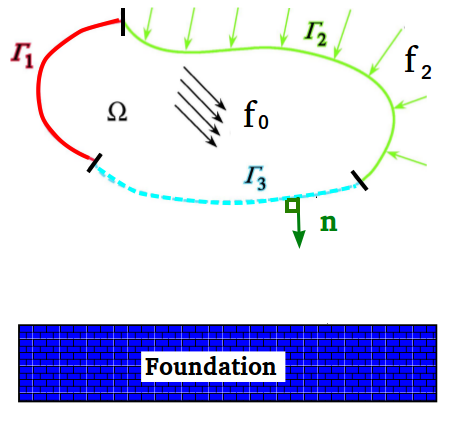
\includegraphics[width=0.4\textwidth]{chapitres/chapitre_2/figures/fig_deformable_1.png}}
\hspace{\fill}
   \subfloat[\label{setting_2} ]{%
      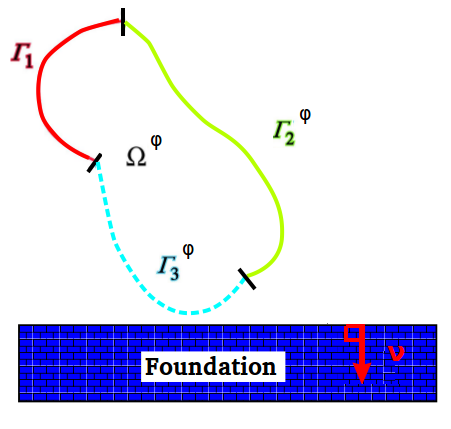
\includegraphics[width=0.4\textwidth]{chapitres/chapitre_2/figures/fig_deformable_2.png}}\\
\caption{Cadre physique (a) de référence et (b) déformée du corps déformable en contact avec une fondation rigide.}
\label{setting}
\end{figure*}
%ffffffffffffffffffffffffffffff


Le corps hyper-élastique est sous l'action des forces volumiques de densité $\fb_0$ et de tractions de surface de densité $\fb_2$
qui agissent sur $\Gamma_2$. Dans le reste du chapitre, nous considérons l'intervalle de temps d'intérêt $[0,T]$ avec $T>0$. On dénote par $t\in [0,T]$ la variable de temps, et, comme mentionné précédemment, $\bx\in \Omega\cup\Gamma$ représentera la variable spatiale. Afin de simplifier la notation, nous n'indiquons pas la dépendance des fonctions par rapport à $\bx$ et $t$. De plus, la notation $\dot\square$ représente la dérivée par rapport au temps de la fonction $\square$. Nous supposons également que le corps est fixé sur $\Gamma_1$ et peut entrer en contact en $\Gamma_3$ avec la fondation. Dans le problème ci-dessous, les conditions de contact avec frottement sont basées sur la combinaison des conditions de contact unilatéral avec une loi de Coulomb de frottement sec sur $\Gamma_3$. Nous désignons par $\bphi:[0,T]\times\overline{\Omega}\to\mathbb{R}^d$ le champ des déformations, en ce sens que $\bphi(t,x)=\bx+\bu(t,x)$ est la position à l'instant $t\in[0,T]$ du point $x\in\overline{\Omega}$. Pour tout point $x\in\Gamma_3$, on définit le point $\overline{y}(x)$ de la fondation, le plus proche de x:

\begin{eqnarray*}
\overline{y}(t,x)=\argmin_{y\in foundation}||\bphi (t,x)-y||_2,
\end{eqnarray*}

De cette façon, on peut définir la distance de contact minimale permise (gap) entre un point de $\Gamma_3$ est sa projection orthogonale sur la fondation rigide comme suit:

\begin{eqnarray*}
d_{\nu}=(\bphi(t,x)-\overline{y}(t,x))\cdot\bnu, \quad \forall x \in \Gamma_3
\end{eqnarray*}

\noindent où $\bnu$ est le vecteur normal unitaire interne à la fondation rigide. La force normale de contact $\Pi_\nu$, supposée négative peut s'écrire dans la direction $\bnu$:

\begin{eqnarray*}
\Pi_\nu=\bnu \cdot \bPi \bn,
\end{eqnarray*}

De la même façon, la force de frottement peut également s'exprimer en fonction du premier tenseur de Piola-Kirchhoff:

\begin{eqnarray*}
\bPi_{\tau}=\bPi-\Pi_{\nu} \bnu,
\end{eqnarray*}

Avec ces définitions mises en places, la vitesse de contact tangentielle $\dot{\bu}_\tau$ d'un point $x\in \Gamma_3$, relative à la surface opposée de la fondation, est donnée de la façon suivante:

\begin{eqnarray*}
\dot{\bu}_\tau=[\bI_d-\bnu \otimes \bnu]\dot{\bu} (t,x),
\end{eqnarray*}

Les conditions de contact unilatéral sur $\Gamma_3$ dépendent du déplacement normal $u_\nu$ et de la contrainte normale $\Pi_\nu$ et sont décrites par les conditions suivantes:

\begin{eqnarray}
d_{\nu}\le 0,\quad \Pi_\nu\le 0, \quad d_{\nu}\Pi_\nu=0,
\end{eqnarray}

Pour plus de détails sur les grands déplacements en contact avec frottement glissants entre les solides déformables, voir \cite{poulios2015unconstrained}.\\

{\bf Remarque:} \textit{Selon le choix du vecteur normal entre $\Gamma_3$ et la fondation rigide au point considéré, on peut écrire la loi de contact unilatéral avec interstice sous la forme  $d_{\nu}\le 0$. Un autre choix de normale amènerait à considérer plutôt  $d_{\nu}\ge 0$. Dans les 2 cas, les démonstrations restent très similaires.}\\

La loi de frottement de Coulomb dépend de la contrainte de frottement tangentielle $\bPi_\tau $, de la pression de contact normale $\Pi_\nu$ et de la vitesse de contact tangentielle $ \dot \bu_{\tau}$ par ces relations:

\begin{eqnarray}
&& \|\bPi_\tau\|\le\mu\,|\Pi_\nu|,\\[2mm]
&& -\bPi_\tau=\mu\,|\Pi_\nu|\,\frac{{\dot\bu}_\tau}{\|{\dot\bu}_\tau\|} \ \ {\rm si}\ \ \dot{\bu}_\tau\ne\bzero,
\end{eqnarray}

\noindent où $\mu$ dénote le coefficient de frottement.

\noindent Avec ces notations, la formulation du problème de contact dynamique dans le cadre de l'hyper-élasticité que nous considérons dans ce travail est la suivante.

\medskip\noindent
{\bf Problème} ${\cal P}$. {\it Trouver le champ de déplacement
$\bu:\Omega\times [0,T]\to\mathbb{R}^d$ et le champ de contrainte
$\boldsymbol{\Pi}:\Omega\times [0,T]\to\mathbb{M}^d$ tel que}
\begin{eqnarray}
\label{1} \boldsymbol{\Pi}=\partial_{\bf F} W({\bf F})\quad&{\rm dans}\
&\Omega\times(0,T),\\[3mm]
\label{2} -\rho\ddot{\bu} + {\rm Div}\,\boldsymbol{\Pi}+\fb_0=\bzero\quad&{\rm
dans}\ &\Omega\times(0,T),\\[3mm]
\label{3} \bu=\bzero\quad &{\rm sur}\ &\Gamma_1\times(0,T),\\[3mm]
\label{4} \boldsymbol{\Pi}\bnu=\fb_2\quad&{\rm sur}\
&\Gamma_2\times(0,T),\\[3mm]
\label{5} d_{\nu}\le 0,\quad
\Pi_\nu\le 0,\quad d_{\nu}\Pi_\nu=0\quad
&{\rm sur}&\ \Gamma_3\times(0,T), \\[3mm]
\label{6}
\left\{\begin{array}{ll}
\|\bPi_\tau\|\le\mu\,|\Pi_\nu|,\\[2mm]
-\bPi_\tau=\mu\,|\Pi_\nu|\,\frac{{\dot\bu}_\tau}{\|{\dot\bu}_\tau\|}
\ \ {\rm si}\ \ \dot{\bu}_\tau\ne\bzero.
\end{array}\right. \quad
&\mbox{sur}&\ \Gamma_3\times(0,T), \\[2mm]
\bu(0)=\bu_0,\ \dot{\bu}(0)=\bu_1 \quad &{\rm dans}&\ \Omega.
\label{p:7}
\end{eqnarray}

Les conditions de compatibilité sur le déplacement initial sont écrites comme suit $\boldsymbol{\Pi}(\bx,0)=\partial_{\bf F} W(\bx,{\bf I} + \nabla {\bu}(\bx,0))$. L'équation (\ref{1}) représente la loi de comportement hyper-élastique du matériau. L'équation (\ref{2}) représente l'équation du mouvement dans laquelle $\rho $ représente la densité du matériau et est supposée constante, par souci de simplicité. Les conditions (\ref{3}), (\ref{4}) représentent respectivement les conditions aux limites de déplacement et de traction.
Enfin, les conditions (\ref{5}) et (\ref{6}) représentent les conditions de contact et de frottement décrites précédemment dans cette section. A noter que les conditions (\ref{5}) sont équivalentes à l'inclusion sous-différentielle suivante (cf \cite{moreau1977application})
\begin{equation}\label{10n}
-\Pi_{\nu} \in \partial \Psi_{\RR^-}(d_{\nu})\quad sur \quad \Gamma_3\times(0,T),
\end{equation}
où $\partial$ représente l'opérateur sous différentiel au sens de l'analyse convexe et $\Psi_A$ désigne la fonction indicatrice de l'ensemble $A \subset \mathbb{R}$.
Une considération similaire pour la contrainte de frottement conduit à
\begin{equation}\label{incluCoul0}
-\bPi_{\tau}\in -\mu\Pi_{\nu}\partial\|{\dot\bu}_{\tau}\|
\quad{\rm sur}\ \Gamma_3\times(0,T),
\end{equation}
ce qui équivaut à (\ref{6}). Enfin, (\ref{p:7}) représente les conditions initiales dans lesquelles $\bu_0$ et $\bu_1$ sont respectivement le déplacement et la vitesse initiaux.

\medskip

\subsection{Formulation variationelle}

Afin d'écrire la formulation variationnelle du problème $ {\cal P} $, des notions préliminaires doivent être précisées. Les notations standard pour les espaces de Sobolev et Lebesgue associées à $\Omega$
et $\Gamma$ sont utilisées. Les espaces suivants considérés ci-dessous
$$
V=\{\bv\in W^{1,s}(\Omega;\mathbb{R}^d)\,\,:\,\,\bv=0\,\,\,\text{sur}\,\,\,\Gamma_1\};\,\,\,\,s > 2.
$$
sont des espaces fonctionnels dotés de leur produits scalaires classiques $(\bu,\bv)_V$ et $(\boldsymbol{\Pi},\btau)_H$ et de leurs normes associées $\|\cdot\|_{V}$ et $\|\cdot\|_{H}$, respectivement. Notons que
$V\subset H\subset V^*$ est un triplet d'évolution, tous les plongements étant continus, compacts et denses. La dualité entre $V^*$ et $V$ sera désigné par
$\langle\bu,\bv\rangle_{{V^*}\times{V}}$. Nous définissons également $W = \{ \bv \in H^{1}(\Omega;\mathbb{R}^d)\, : \, \bv=\bzero\ \ \textrm{sur}\ \ \Gamma_1 \} $. Clairement, $V\subset W \subset H \subset W^*\subset V^*$, tous les plongements étant continus.\\

Notons que, pour plus de commodité, les multiplicateurs de Lagrange $\lambda_{\nu}$ et $\blambda_{\tau}$ sont pris égaux à $-\Pi_{\nu}$ et $-\bPi_{\tau}$, respectivement. À cette effet, nous avons défini par
$X_\nu=\left\{\,v_\nu|_{\Gamma_3} : \ \bv \in V\, \right\}$ et
$X_\tau=\left\{\,\bv_\tau|_{\Gamma_3} : \ \bv \in V\, \right\}$
les traces d'espaces munies de leurs normes habituelles. Nous désignons par $Y_\nu$ et $Y_\tau$ les duals des espaces $X_\nu$ et $X_\tau$, respectivement. De plus, nous désignons par
$\langle\cdot,\cdot\rangle_{Y_{\nu},X_{\nu}}$ et $\langle\cdot,\cdot\rangle_{Y_{\tau},X_{\tau}}$la paire duale correspondante. Ensuite, une fonction $\varphi_\nu :
X_\nu\to[0,+\infty]$ est introduite, définie par
\begin{eqnarray*}
&&\varphi_\nu(v_\nu) = \int_{\Gamma_3} \Psi_{\RR^-}(v_\nu)\,d\Gamma
\quad \forall\, v_\nu \in X_\nu.
\end{eqnarray*}
Par conséquent, le multiplicateur de Lagrange $\lambda_{\nu}$ lié à la contrainte de contact vérifie une inclusion sous différentielle étendue dérivant de l'inclusion sous différentielle ponctuelle définie dans (\ref{10n}).
\begin{equation}
\label{signsub} \lambda_\nu \in
\partial\varphi_\nu(d_{\nu}) \quad {\rm
dans}\quad Y_{\nu}.
\end{equation}
De manière similaire, nous introduisons une fonction $\varphi_\tau:X_{\tau}\to[0,+\infty]$ définie par
\begin{eqnarray*}
&&\varphi_\tau(\bv_\tau) = \int_{\Gamma_3}\|{\dot\bv}_{\tau}\|\,d\Gamma
\quad \forall\, \bv_\tau \in X_\tau,
\end{eqnarray*}
et, par suite, la condition (\ref{incluCoul0}) conduit à l'inclusion sous différentielle étendue suivante
\begin{equation}\label{incluCoul}
\blambda_{\tau}\in \mu\lambda_{\nu}\partial\varphi_\tau({\bu}_{\tau}) \quad {\rm
dans}\quad Y_{\tau}.
\end{equation}
Aussi, pour une fonction de contrainte régulière $\boldsymbol{\Pi}$, la formule de Green suivante est valable:
\begin{equation}
\int_\Omega\,\boldsymbol{\Pi}:\nabla\bv\,dx+\int_\Omega\,{\rm
Div}\,\boldsymbol{\Pi}\cdot\bv\,dx = \int_\Gamma\boldsymbol{\Pi}\bn \cdot\bn\,da
\quad {\rm\ pour\ tout }\ \bv\in H_1. \label{Green}
\end{equation}
\noindent De plus, dans l'étude du problème mécanique (\ref{1})--(\ref{6}), nous supposons que les forces surfaciques et les densités de traction sont régulières
\begin{eqnarray}
\label{f} 
  &&  \fb_0 \in L^2(0,T;L^{p_1}(\Omega)), \qquad \fb_2\in L^2(0,T;L^{p_2}(\Gamma_2)), \\
  &&   \textrm{où} \qquad p_1\begin{cases}
    \in (1,\infty) &\textrm{si}\quad d=2,\\
   =\frac{6}{5}&\textrm{si}\quad d=3,
    \end{cases}\quad\textrm{et}\quad p_2\begin{cases}
         \in (1,\infty) &\textrm{si}\quad d=2,\\
      = \frac{4}{3}&\textrm{si}\quad d=3 .
        \end{cases} \nonumber 
\end{eqnarray}
Nous passons maintenant à la formulation variationnelle hybride du problème ${\mathcal
P}$. À cet effet, nous introduisons l'élément $\fb$ défini par

\begin{eqnarray}
&&\label{ff}(\fb(t),\bv)_V=(\fb_0(t),\bv)_H+(\fb_2(t),\bv)_{L^2(\Gamma_2)},\qquad\forall\bv\in V.
\end{eqnarray}
En utilisant la dualité entre $ V ^ * $ et $ V $, la formule de Green (\ref{Green}) et la définition (\ref{ff}), nous obtenons la relation suivante
\begin{eqnarray}
&& \langle{\rho\ddot{\bu}(t),\bv}\rangle_{{V^*}\times{V}} + \label{x1}\langle{\boldsymbol{\Pi},\nabla\bv}\rangle_{{V^*}\times{V}}=(\fb(t),\bv)_V
+\int_{\Gamma_3}\,\Pi_\nu
v_\nu\,da+\int_{\Gamma_3}\,\boldsymbol{\Pi}_\tau\cdot\bv_\tau\,da.\nonumber
\end{eqnarray}
Ensuite, en utilisant le multiplicateur de Lagrange $\lambda_{\nu}$, lié à la contrainte de contact normale $\Pi_{\nu}$, et le multiplicateur de Lagrange $\blambda_{\tau}$, lié à la contrainte de contact tangentielle $\bPi_{\tau}$, nous obtenons la formulation variationnelle du problème de contact avec frottement ${\cal P}$ en termes de deux champs inconnus.\\

{\textbf{Problème}\ ${\cal P}_V$}
{\it Trouver le champ de déplacement $\bu \in L^\infty(0,T;V)$, avec $\dot\bu \in L^2(0,T;W)$ et $\ddot\bu \in L^2(0,T;V^*)$, le champ de contrainte normal $\lambda_{\nu}: [0,T]\rightarrow Y_\nu$ et le champ de contrainte tangentiel $\blambda_{\tau} : [0,T]\rightarrow  Y_\tau$ tel que $\forall\,\bv\in V$}
\begin{eqnarray}\label{weak0}\label{10}
&\hspace{-5mm} {\footnotesize\langle{\rho\ddot{\bu}(t),\bv}\rangle_{{V^*}\times{V}}+ \langle{\boldsymbol{\Pi},\nabla\bv}\rangle_{{V^*}\times{V}} +\langle \lambda_{\nu}(t),v_{\nu}\rangle_{Y_{\nu},X_{\nu}}+\langle \blambda_{\tau}(t),\bv_{\tau}\rangle_{Y_{\tau},X_{\tau}}=(\fb(t),\bv)_V,}\\
\label{weak}
&\label{10bis}\lambda_{\nu}(t) \in
\partial\varphi_\nu(d_{\nu})\quad {\rm dans}\ Y_\nu,\\
&\label{10ter}\blambda_{\tau}(t) \in \mu\lambda_{\nu}\partial\varphi_\tau({\bu}_{\tau}) \quad {\rm dans}\ Y_{\tau},
\end{eqnarray}{\it pour
	tout} $t\in [0,T]$ {\it et, de plus,}
\begin{equation}\label{BDSxx}
\bu(0)=\bu_0,\qquad\dot\bu(0)=\bu_1.
\end{equation}

Une paire $(\bu,\blambda)$ qui satisfait (\ref{10}), (\ref{10bis}), (\ref{10ter}) avec la loi de comportement hyper-élastique sous la forme $\boldsymbol{\Pi}=\partial_{\bf F} W({\bf F})$ est appelée {\it solution faible} du problème variationnel de contact de frottant ${\cal P}_V$. Voir \cite{ciarlet1988mathematical}, \cite{le1994numerical} et \cite{barboteu2018analysis} pour plus de détails sur l'analyse de la formulation variationnelle des problèmes d'hyper-élasticité.

\section{Approximation variationnelle}\label{approx_var}

Cette section est consacrée à la discrétisation du problème variationnel ${{\mathcal P}}_V$, basée sur des arguments similaires à ceux utilisés dans \cite{ayyad2009formulation,ayyad2009frictionless,barboteu2013analytical,barboteu2015dynamic,barboteu2014analysis,khenous2006hybrid,khenous2006discretization}. Tout d'abord, nous rappelons quelques éléments préliminaires concernant l'étape de discrétisation temporelle. Soit $ N $ un entier, et $\Delta t=\frac{T}{N}$ un pas de temps. Nous considérons une collection discrète de temps: 
\[ t_n=n\,\Delta t,\quad 0\le n\le N. \]
Pour une fonction $f$ continue par rapport au temps, nous utiliserons la notation $f_j=f(t_j)$ pour $0 \leq j \leq N$. Dans ce qui suit, nous considérons une collection de temps discrets $\{t_n\}_{n=0}^{N}$ qui définit une partition uniforme de l'intervalle de temps $[0,T]= \bigcup_{\scriptstyle n=1}^{N}[t_{n-1},t_{n}]$, avec $t_0=0$, $t_{n}=t_{n-1} + \Delta t$ et $t_N=T$. Finalement, pour une suite $\{w_n\}_{n=1}^N$, nous désignons les différences divisées de point milieu par

\begin{equation}\label{midp}
\dot w_{n-\frac{1}{2}}=(w_{n}-w_{n-1})/\Delta t = \frac{1}{2}(\dot w_{n} + \dot w_{n-1}),
\end{equation}

et, de manière équivalente, nous avons $\dot w_{n}=-\dot
w_{n-1}+\frac{2}{\Delta t}(w_{n}-w_{n-1})$. Ensuite, nous utilisons la notation $\Box_{n-\frac{1}{2}} = \frac{1}{2}(\Box_n +
\Box_{n-1})$, où $\Box_n$ représente l'approximation de
$\Box(t_n)$. Notons que le schéma d'intégration en temps que nous utilisons est basé sur un schéma implicite d'ordre 2 que l'on retrouve dans (\ref{midp}).\\
Nous présentons maintenant quelques éléments concernant l'étape de discrétisation spatiale. Soit $\Omega$ un domaine polyédrique. Considérons une partition régulière $\{{\cal T}^h\}$ d'éléments finis triangulaires de $\overline {\Omega}$ qui sont compatibles avec la décomposition des frontières
$\Gamma=\overline{\Gamma_1}\cup\overline{\Gamma_2}\cup\overline{\Gamma_3}$, i.e., si un côté d'un élément $Tr\in{\cal T}^h$ a plus d'un point sur $ \Gamma $, alors le côté repose entièrement sur $\overline{\Gamma_1}$, $\overline{\Gamma_2}$ ou
$\overline{\Gamma_3}$. L'espace $V$ est approché par l'espace de dimension finie $V^h \subset V$ des fonctions continues et affines par morceaux, c'est-à-dire:

\begin{eqnarray}
&& \hspace*{-0.7cm}V^h=\{\,\bv^h\in [C(\overline{\Omega})]^d \; :
\; \bv^h|_{Tr}\in [P_1(Tr)]^d \,
\,\,\,   \forall\,Tr\in {\T}^h, \nonumber\\
 && \qquad \qquad \quad \bv^h=\bzero \,\,\, \hbox{aux noeuds sur}\,\,\, \Gamma_1\,\},\nonumber
\end{eqnarray}

où $P_1(Tr)$ représente l'espace des polynômes de degré inférieur ou égal à 1 dans $Tr$ et $h>0$ désigne le paramètre de discrétisation spatiale. Pour la discrétisation des espaces de multiplicateurs de Lagrange $Y_{\nu}$ et $Y_{\tau}$, nous utilisons des fonctions constantes par morceaux comme cela se fait dans \cite{barboteu2015hyperelastic}.
Les espaces multiplicateurs de Lagrange discrets sont désignés par $Y_{\nu}^h$ et $Y_{\tau}^h$. Plus de détails sur l'étape de discrétisation peuvent être trouvés dans \cite{khenous2006discretization,khenous2006hybrid,wriggers2004computational}.\\

Les éléments $\bu^h_0 \in V^h$ et $\bu^h_1 \in V^h$ sont des éléments discrets issus de l'approximation d'éléments finis de $\bu_0$ et $\bu_1$, respectivement. Ensuite, en utilisant les notations précédentes et le schéma point milieu (\ref{midp}), l'approximation discrète du problème ${{\mathcal P}}_V$ au temps $t_{n-\frac{1}{2}}$ est comme suit. Ici, nous utilisons une différence divisée implicite rétrograde pour la discrétisation de la vitesse tangentielle $\dot\bu_\tau(t)$ donnée par $ \dot{{\bu}_\tau}_{n-\frac{1}{2}} = ({\bu_\tau}_n - {\bu_\tau}_{n-1})/\Delta t$, ce qui conduit au problème discret suivant.

\medskip \noindent{\bf Problème} ${\mathcal P}_V^{h\Delta t}$. {\it
	Trouver un champ de déplacement discret
	$\bu^{h\Delta t}=\{\bu_n^{h\Delta t}\}_{n=0}^N\subset V^h$, un champ de contrainte normale discret $\lambda_{\nu}^{h\Delta t} =\{{\lambda_{\nu}}_{n}^{h\Delta t}\}_{n=0}^N
	\subset Y^h_\nu$ et un champ de contrainte tangentielle discret
	$\bxi_{\tau}^{h\Delta t} =\{{\bxi_{\tau}}_{n}^{h\Delta t}\}_{n=0}^N \subset
	Y^h_\tau$ tel que, pour tout $n=1,\ldots,N$,}
%%%%%%%%%%%%%%%%%%%%%
\begin{eqnarray}
&&   \dual{{\rho}{\ddot{\bu}^{h\Delta t}_{n-\frac{1}{2}}},\bv^h}{V} + \dual{\boldsymbol{\Pi},\nabla\bv^h}{V} +   \langle {\lambda_{\nu}}^{h\Delta t}_{n-\frac{1}{2}},v^h_{\nu}\rangle_{Y^h_\nu,X^h_\nu} + \langle
{\blambda_{\tau}}^{h\Delta t}_{n-\frac{1}{2}},v^h_{\tau}\rangle_{Y^h_\tau,X^h_{\tau}} \nonumber  \\[2mm]
&&
\qquad \qquad \qquad \qquad \qquad \qquad =  \dual{\fb^{h\Delta t}_{n-\frac{1}{2}},\bv^h}{V} \quad
\forall\,\bv\in V^h, \label{LMh} \\[2mm]
&&\label{LMch} -{\lambda_{\nu}}^{h\Delta t}_{n-\frac{1}{2}}\in
\partial\varphi_\nu({d_{\nu}}^{h\Delta t}_{n-\frac{1}{2}}),\\[2mm]
&&\label{LMfh} -{\blambda_{\tau}}^{h\Delta t}_{n-\frac{1}{2}}\in -\mu  {\lambda_\nu}^{h\Delta t}_{n-\frac{1}{2}} \partial\varphi_\tau(\dot{{\bu}_{\tau}}^{h\Delta t}_{n-\frac{1}{2}}),\\[2mm]
&&\label{cih1} \bu^{h\Delta t}_{0}=\bu^{h}_{0}, \quad\quad
\delta\bu^{h\Delta t}_{0}=\bu^{h}_{1}.
\end{eqnarray}
%%%%%%%%%%%%%%%%%%%%%
%*********************************
où $\ddot{\bu}^{h\Delta t}_{n-\frac{1}{2}} = \frac{\dot{\bu}^{h\Delta t}_{n}-\dot{\bu}^{h\Delta t}_{n-1}}{\Delta t}$ est l'approximation de l'accélération ${\ddot\bu}$ au temps $t_{n-\frac{1}{2}}$.\\

En partant du problème ${\mathcal P}_V^{h\Delta t}$ et en utilisant le formalisme introduit dans \cite{pietrzak1999large} et \cite{laursen2013computational} basé sur l'approximation de Galerkin pour l'hyper-élasticité, nous poserons directement le problème élémentaire discret fort comme suit.

\medskip \noindent{\bf Problème} ${\mathcal P}_S^{nodal}$. {\it
	Trouver un vecteur de déplacement global
	$\bu^{\Delta t}=\{\bu_n^{\Delta t}\}_{n=0}^N$, un vecteur de contrainte normal global $\lambda_{\nu}^{\Delta t} =\{{\lambda_{\nu}}_{n}^{\Delta t}\}_{n=0}^N$ et un vecteur de contrainte tangentiel global
	$\blambda_{\tau}^{\Delta t} =\{{\blambda_{\tau}}_{n}^{\Delta t}\}_{n=0}^N$ tel que, pour tout $n=1$}
%%%%%%%%%%%%%%%%%%%%%
\begin{eqnarray}
&&   \rho \ddot{\bu}^{\Delta t}_{n-\frac{1}{2}} + A(\bu^{\Delta t}_{n-\frac{1}{2}}) + {\lambda_{\nu}}^{\Delta t}_{n-\frac{1}{2}}\bnu + {\blambda_{\tau}}^{\Delta t}_{n-\frac{1}{2}}- \fb = \bzero \nonumber  \\[2mm]
&&\label{LMch2} -{\lambda_{\nu}}^{\Delta t}_{n-\frac{1}{2}}\in
\partial\varphi_\nu({d_{\nu}}^{\Delta t}_{n-\frac{1}{2}}),\nonumber\\[2mm]
&&\label{LMfh2} -{\blambda_{\tau}}^{\Delta t}_{n-\frac{1}{2}}\in -\mu  {\lambda_\nu}^{\Delta t}_{n-\frac{1}{2}} \partial\varphi_\tau(\dot{{\bu}_{\tau}}^{\Delta t}_{n-\frac{1}{2}}), \nonumber\\[2mm]
&&\label{cih12} \bu^{\Delta t}_{0}=\bu_{0}, \quad\quad
\delta\bu^{\Delta t}_{0}=\bu_{1}.\nonumber
\end{eqnarray}
%%%%%%%%%%%%%%%%%%%%% 
où $A(.)$ est le vecteur de force interne provenant du premier tenseur de Piola-Kirchhoff ${\Pi}$.\\
Par la suite, pour simplifier la notation et la lisibilité, nous n'indiquons pas la dépendance des variables par rapport aux paramètres de discrétisation $\Delta t$ et
$h$. Par exemple, nous écrirons $\bu$ au lieu de $\bu^{h\Delta t}_{n-\frac{1}{2}}$.\\
	
\textbf{Dans les sections qui suivent, nous allons proposer à la fois la méthode semi-régulière de Newton ainsi que l'algorithme PDAS pour chaque cas de contact, à savoir: la loi de contact unilatéral sans frottement (Section 4), la loi de contact bilatéral avec frottement de Tresca (Section 5) et la loi de contact unilatéral avec frottement de Coulomb (Section 6 et 7).}	

\section{Loi de contact unilatéral sans frottement avec interstice}\label{uni_frictionless}
Dans un premier temps, nous considérons une loi de contact unilatéral sans frottement avec interstice.
Notant par $p$ l'indice des sommets sur $\Gamma_3^h \in \Gamma_3$ et avec ces considérations, les conditions unilatérales discrètes vérifiées sur la frontière de contact $\Gamma_3^h$ sont données par

\begin{eqnarray}
&&\label{nudc}d_{\nu,p}\le 0,\\[2mm]
&&\label{lmbnudc}\lambda_{\nu, p}\ge 0,\\[2mm]
&&\label{unulmbddc}d_{\nu,p}\lambda_{\nu, p}= 0,\\[2mm]
&&\label{lmbddf} \blambda_{\tau, p}= \bzero.
\end{eqnarray}

\subsection{Approche de Newton semi-régulière}\label{Activeset_type}

\subsubsection{Fonction de complémentarité de contact}\label{comp_cont}

\noindent Dans ce paragraphe, nous allons réécrire les conditions de contact unilatéral de Signorini (\ref{nudc})--(\ref{unulmbddc}) à l'aide d'une fonction de complémentarité non-linéaire de contact unilatéral 
\begin{align}\label{phi1c}
{\cal R}_{\nu}^{\blambda}(u_{\nu, p},\lambda_{\nu, p})=\lambda_{\nu, p}-\max(0,\lambda_{\nu, p}+c_{\nu}d_{\nu,p}).
\end{align}

\begin{proposition}\label{prop1}
Soit $c_\nu>0$, les conditions de contact unilatéral de Signorini (\ref{nudc})--(\ref{unulmbddc}) sont équivalentes à la relation ${\cal R}_{\nu}^{\blambda}(u_{\nu, p},\lambda_{\nu, p})=0$
\begin{align*}\label{phi1c}
{\cal R}_{\nu}^{\blambda}(u_{\nu, p},\lambda_{\nu, p})=\lambda_{\nu, p}-\max(0,\lambda_{\nu, p}+c_{\nu}d_{\nu,p}).
\end{align*}
\end{proposition}
\noindent
\textit{Preuve.} Supposons que les conditions de Signorini (\ref{nudc})--(\ref{unulmbddc}) soient vérifiées. Alors, soit $d_{\nu,p} < 0$, soit $d_{\nu,p} = 0$. Si $d_{\nu,p} < 0$, la condition (\ref{unulmbddc}) implique que $\lambda_{\nu, p} = 0$. Alors\\
\begin{equation*}
-\max(0,\lambda_{\nu, p}+c_{\nu}d_{\nu,p}) = -\max(0,c_{\nu}d_{\nu,p}) = 0.\\
\end{equation*}
\noindent
Supposons maintenant que $d_{\nu,p} = 0$, et $\lambda_{\nu, p} > 0$, on a alors\\
\begin{equation*}
-\max(0,\lambda_{\nu, p}+c_{\nu}d_{\nu,p}) = -\max(0,\lambda_{\nu, p}) = -\lambda_{\nu, p}.\\
\end{equation*}
Réciproquement, si (\ref{phi1c}) est vérifiée, cela implique que 
(\ref{lmbnudc}) est également vérifiée. Si $\lambda_{\nu, p} = 0$, nous avons,\\
\begin{equation*}
-\max(0,c_{\nu}d_{\nu,p}) = 0,\\
\end{equation*}
\noindent
Ce qui veut dire que $d_{\nu,p} < 0$, puisque $c_{\nu} > 0$. Finalement, si $\lambda_{\nu, p} > 0$,\\ $\lambda_{\nu, p}+c_{\nu}d_{\nu,p} > 0$ et\\
\begin{equation*}
{\cal R}_{\nu}^{\blambda}(u_{\nu, p},\lambda_{\nu, p})=\lambda_{\nu, p}-\lambda_{\nu, p}+c_{\nu}d_{\nu,p} = c_{\nu}d_{\nu,p} = 0,\\
\end{equation*}
\noindent
et comme $c_{\nu} > 0$, alors $d_{\nu,p} = 0$. Par suite, (\ref{nudc})--(\ref{unulmbddc}) sont vérifiées, ce qui conclut la preuve.

\subsubsection{Dérivée généralisée de la fonction de complémentarité}\label{gen_deriv}

Maintenant, nous allons déterminer la dérivée généralisée de la fonction de complémentarité dans les cas d'interstice et de contact.\\

$\bullet$ \underline{Statut non contact: $\lambda_{\nu, p}+c_{\nu}d_{\nu,p}\le 0$}

\noindent Dans ce cas, la fonction de complémentarité devient:
\begin{align*}
&{\cal R}_{\nu}^{\blambda}(u_{\nu, p},\lambda_{\nu, p})=\lambda_{\nu, p}.
\end{align*}
Ensuite, il est évident de voir que
\begin{align}
&d_{u_{\nu, p}} {\cal R}_{\nu}^{\blambda}=0\label{phi11c},\\
&d_{\lambda_{\nu, p}} {\cal R}_{\nu}^{\blambda}=d{\lambda_{\nu, p}}\label{phi12c}.
\end{align}

$\bullet$ \underline{Statut contact: $\lambda_{\nu, 
p}+c_{\nu}d_{\nu,p}> 0$}\\
\noindent On a:
\begin{align*}
&{\cal R}_{\nu}^{\blambda}(u_{\nu, p},\lambda_{\nu, p})=-c_{\nu}d_{\nu,p}.
\end{align*}
Alors, on peut vérifier que
\begin{align}
&d_{u_{\nu, p}} {\cal R}_{\nu}^{\blambda}=-c_{\nu}d{u_{\nu, p}}\label{phi11stc},\\
&d_{\lambda_{\nu, p}} {\cal R}_{\nu}^{\blambda}=0\label{phi12stc}.
\end{align}
\noindent En combinant (\ref{phi11c}) -- (\ref{phi12stc}) avec ${\cal G}_{{\cal R}_{\nu}^{\blambda}}$ la dérivée généralisée de ${\cal R}_{\nu}^{\blambda}$, nous obtenons
\begin{align}
&{\cal G}_{{\cal R}_{\nu}^{\blambda}}(u_{\nu, p},\lambda_{\nu, p})(\delta u_{\nu, p},\delta\lambda_{\nu, p})= -c_{\nu}(1-{\cal X}_{Gap})\delta u_{\nu, p} + {\cal X}_{Gap} \delta\lambda_{\nu, p},\label{derivgen}
\end{align}
où 
\begin{align*}
&{\cal X}_{Gap} =1, \ {\rm si}\ \lambda_{\nu, p}+c_{\nu}d_{\nu,p}\le 0,\\
&{\cal X}_{Gap} =0,  \ {\rm si}\ \lambda_{\nu, p}+c_{\nu}d_{\nu,p}> 0.
\end{align*}
En utilisant maintenant le formalisme semi-régulier de Newton sur $(u_{\nu, p}^{(k)},\lambda_{\nu, p}^{(k)})$ à partir de la dérivée généralisée (\ref{derivgen}), nous pouvons en déduire le nouveau couple d'itéré $(u_{\nu, p}^{(k+1)},\lambda_{\nu, p}^{(k+1)})$ avec le schéma itératif d'indice $k$ suivant: 
\begin{align}
&{\cal G}_{{\cal R}_{\nu}^{\blambda}}(u_{\nu, p}^{(k)},\lambda_{\nu, p}^{(k)})(\delta u_{\nu, p}^{(k+1)},\delta\lambda_{\nu, p}^{(k+1)})= - {\cal R}_{\nu}^{\blambda} (u_{\nu, p}^{(k)},\lambda_{\nu, p}^{(k)})\label{phi21c},\\
& \mbox{où} \qquad (u_{\nu, p}^{(k+1)},\lambda_{\nu, p}^{(k+1)}) = (u_{\nu, p}^{(k)},\lambda_{\nu, p}^{(k)}) + (\delta u_{\nu, p}^{(k+1)},\delta \lambda_{\nu, p}^{(k+1)})\label{phi22c}
\end{align}

$\bullet$ \underline{Statut non contact: ${\cal X}_{Gap} =1$}

\noindent A partir de (\ref{phi11c}), (\ref{phi12c}), (\ref{phi21c}) et (\ref{phi22c}), il vient
\begin{align}
&\lambda_{\nu, p}^{(k+1)}-\lambda_{\nu, p}^{(k)}=-\lambda_{\nu, p}^{(k)}.
\end{align}
Ensuite,
\begin{align}
&\lambda_{\nu, p}^{(k+1)}=0,\label{lambdanukp1}
\end{align}

$\bullet$ \underline{Statut contact: ${\cal X}_{Gap} =0$}

\noindent En combinant (\ref{phi11stc}),  (\ref{phi12stc}), (\ref{phi21c}) et (\ref{phi22c}), on a
\begin{align}
&-c_\nu \delta u^{(k+1)}_{\nu,p}=c_{\nu}d_{\nu, p}^{(k)}.
\end{align}
Ensuite,
\begin{align}
&\delta u^{(k+1)}_{\nu,p} = -d^{(k)}_{\nu,p}.\label{unukp1}
\end{align}
 
\subsection{Méthode Primal-Dual Active Set (PDAS)}

Les méthodes de type Active Set ou \textit{"Ensemble Actif"} sont des approches mathématiques utilisées afin de résoudre un problème d'optimisation qui décrit une fonction à minimiser ou maximiser, et un ensemble de contraintes qui définissent la recherche de la solution optimale. Cette approche est particulièrement importante dans la théorie de l'optimisation, car elle détermine les contraintes qui influenceront le résultat final de l'optimisation.\\
Dans l'approche standard PDAS, on distingue les méthodes \textit{Primal Active Set} et \textit{Dual Active Set}. A partir d'un point de départ possible, les méthodes Primal Active Set génèrent une séquence d’itérations réalisables jusqu’à ce que la faisabilité duale soit atteinte, ce qui permet d’obtenir une solution optimale. Les méthodes Dual Active Set pour les problèmes quadratiques convexes génèrent une séquence de double itération réalisable jusqu'à ce que la faisabilité primale soit atteinte, ce qui permet d'obtenir une solution optimale. Plus récemment, des méthodes \textit{Primal-Dual Active Set} (PDAS) ont été envisagées pour résoudre des problèmes variationnels à contraintes unilatérales. Ces approches se caractérisent par le fait que l'ensemble actif est défini par une relation décrite à la fois par la faisabilité primale et duale appliquées ensemble lors de chaque itération.\\

Notons ${\cal S}$  l'ensemble de tous les noeuds du maillage d'éléments finis appartenant à $\Gamma_3^h$ et $p$ l'indice d'un noeud appartenant à ${\cal S}$. Dans ce qui suit, nous utilisons les mêmes notations que dans \cite{hueber2008primal}. Les conditions de contact discrètes (\ref{nudc})--(\ref{unulmbddc}) sont réalisées en appliquant une stratégie d'ensemble actif (Active Set) sur la fonction de complémentarité non-linéaire ${\cal R}_{\nu}^{\blambda}$ basée sur un schéma itératif semi-régulier de Newton. Les ensembles actifs et inactifs sont définis respectivement comme suit
\begin{align}
\left\{\begin{array}{ll}
&{\cal A}_{\nu}^{k+1}=\{p\in {\cal S}:\lambda^{(k)}_{\nu,p}+c_{\nu} d^{(k)}_{\nu,p}> 0\},\\
&{\cal I}_{\nu}^{k+1}=\{p\in {\cal S}:\lambda^{(k)}_{\nu,p}+c_{\nu} d^{(k)}_{\nu,p} \le 0\},.
\end{array}\right.
\label{ensactinact}
\end{align}
Le statut d'un noeud donné à l'itération $k$ dépend de l'ensemble auquel il appartient; il peut être soit dans le statut contact inactif (statut non contact), soit dans le statut contact actif (statut contact) (voir preuve page 24 et (\ref{phi1c})). À chaque incrément $n$ pour le temps $t_{n-\frac{1}{2}}$, nous introduisons également l'opérateur ${\cal R}(.,.)=\left({\cal R}^{\bu}(.,.),{\cal R}_{\nu}^{\blambda}(.,.),{\cal R}_{\tau}^{\blambda}(.,.)\right)$ qui décrit le système d'équations non-linéaires résultant du problème discrétisé ${\mathcal P}_S^{nodal}$ dans le cas d'un contact unilatéral sans frottement, et défini par
\begin{equation}
\label{Rsystem1}
{\cal R}(\bu,\blambda)=\left(
\begin{array}{c}
{\cal R}^{\bu}(\bu,\blambda)=\rho\ddot\bu + A(\bu) + \lambda_{\nu}\bnu - \fb\\[3mm]
{\cal R}_{\nu}^{\blambda}(\bu,\blambda)=\lambda_{\nu, p}-\max(0,\lambda_{\nu, p}+c_{\nu}d_{\nu,p})\\[3mm]
{\cal R}_{\tau}^{\blambda}(\bu,\blambda) = \bzero
\end{array}\right) = \bzero.
\end{equation}

A partir de (\ref{lambdanukp1}), (\ref{unukp1}), (\ref{ensactinact}) et (\ref{Rsystem1}), nous pouvons en déduire l'algorithme itératif de l'ensemble actif d'indice $k$.\\
\qquad(i) Choisir $(\bu^{(0)},\blambda^{(0)})$, $c_{\nu}>0$ et initialiser $k=0$.\\[3mm]
\qquad(ii) Définir les ensembles actifs et inactifs:
\begin{align*}
&{\cal A}_{\nu}^{k+1}=\{p\in {\cal S}:\lambda^{(k)}_{\nu,p}+c_{\nu} d^{(k)}_{\nu,p}> 0\},\\
&{\cal I}_{\nu}^{k+1}={\cal S}\setminus {\cal A}_{\nu}^{k+1}.
\end{align*}
(iii) Trouver $(\bu^{(k+1) },\blambda^{(k+1) })$ tels que
\begin{eqnarray}
&\label{sys_cont}\rho \ddot{\bu}^{(k+1)} + A(\bu^{(k+1)}) + \lambda_{\nu}^{(k+1)}\nu = \fb, \\[1mm]
&\label{Anu_frictionless}\delta u^{(k+1)}_{\nu,p} = -d^{(k)}_{\nu,p} \qquad {\rm pour \ tout} \qquad p\in {\cal A}_{\nu}^{k+1},\\[1mm]
&\label{Inu_frictionless}\lambda^{(k+1)}_{\nu,p}=0 \quad {\rm pour \ tout} \quad p\in {\cal I}_{\nu}^{k+1}.
\end{eqnarray}
(iv) Si $\|(\bu^{(k+1) },\blambda^{(k+1)})-(\bu^{(k) },\blambda^{(k)})\|\leq\epsilon$, $\|{\cal R}(\bu^{(k+1) },\blambda^{(k+1)})\|\leq\epsilon$, ${\cal A}_{\nu}^{k+1}={\cal A}_{\nu}^{k}$  stop, sinon retourner à (ii).\\[1mm]
{\bf Remarque 1:} \textit{Le système non-linéaire (\ref{sys_cont}) correspondant à ${\cal R}^{\bu}(\bu^{(k+1)},\blambda^{(k+1)})=\bzero$ doit être résolu par une méthode de Newton à chaque itération Active Set. Les systèmes linéaires (\ref{Anu_frictionless}) et (\ref{Inu_frictionless}) quant à eux reviennent à écrire la méthode de Newton sur le système à résoudre (\ref{Rsystem1}).}\\

\noindent {\bf Remarque 2:} \textit{Un des aspects les plus intéressants des méthodes PDAS réside dans le fait que les systèmes linéaires qui en sont issus ne nécessitent pas l'utilisation des multiplicateurs de Lagrange et, par conséquent, deviennent plus simple à implémenter puisque les conditions de contact initiales non-linéaires sont remplacées à chaque itération par les conditions linéaires (\ref{Anu_frictionless}) et (\ref{Inu_frictionless}) qui sont respectivement des conditions de Dirichlet et de Neumann.}

\section{Loi de contact bilatéral avec frottement de Tresca}
\label{trescaactive}
Dans cette section uniquement, nous considérons une condition de contact bilatéral combinée à la loi de frottement de Tresca.

Notant par $p$ l'indice des sommets sur $\Gamma_3^h\in \Gamma_3$ et avec ces considérations, les conditions discrètes vérifiées sur la frontière de contact sont données par
\begin{eqnarray}
&&\label{1nudt}u_{\nu, p}=0,\\[2mm]
&&\label{fricdt} \left\{\begin{array}{ll}
\|\blambda_{\tau, p}\|\le\,S,\\[2mm]
\|\blambda_{\tau, p}\|<\,S\Longrightarrow \dot\bu_{\tau, p}=0,\\[2mm]
\|\blambda_{\tau, p}\|=\,S\Longrightarrow \exists \beta\ge 0: \blambda_{\tau, p}=\beta \dot{\bu}_{\tau, p},
\end{array}\right.
\end{eqnarray}
où $S>0$ est un seuil de frottement constant positif.

\subsection{Approche de Newton semi-régulière}\label{Activeset_type}

\subsubsection{Fonction de complémentarité de frottement}\label{comp_cont}

Afin de dériver le schéma itératif, nous introduisons une fonction de complémentarité de frottement de Tresca non-linéaire ${\cal R}_{\tau}^{\blambda}(\dot\bu_{\tau, p},\blambda_{\tau, p})=0$ définie par
\begin{equation}\label{ctresca}
{\cal R}_{\tau}^{\blambda}(\dot\bu_{\tau, p},\blambda_{\tau, p})=\max ( S, \|\blambda_{\tau, p}+c_\tau \dot\bu_{\tau, p}\|)\blambda_{\tau, p}- S (\blambda_{\tau, p}+c_\tau \dot\bu_{\tau, p}).
\end{equation}
Nous allons prouver ce résultat.
\begin{proposition}\label{prop1}
Soit $c_\tau>0$, les conditions de Tresca (\ref{fricdt}) sont équivalentes à la relation ${\cal R}_{\tau}^{\blambda}(\dot\bu_{\tau, p},\blambda_{\tau, p})=0$.
\end{proposition}

\noindent \textit{Preuve.} Supposons (\ref{fricdt}). Tout d'abord, si $\|\blambda_{\tau, p}\|<\,S$, cela implique que $\dot\bu_{\tau, p}=0$. Donc
\begin{equation}
{\cal R}_{\tau}^{\blambda}(\dot\bu_{\tau, p},\blambda_{\tau, p})=\max ( S, \|\blambda_{\tau, p}\|)\blambda_{\tau, p}- S (\blambda_{\tau, p})=0.
\end{equation}
Supposons à présent que $\|\blambda_{\tau, p}\|=\,S$ et $\blambda_{\tau, p}=\beta \dot\bu_{\tau, p}$ avec $\beta>0$; alors
\begin{equation}
{\cal R}_{\tau}^{\blambda}(\dot\bu_{\tau, p},\blambda_{\tau, p})=\max ( S, (\beta +c_\tau)\| \dot\bu_{\tau, p}\|)\beta \dot\bu_{\tau, p}-\beta\|\dot\bu_{\tau, p}\| (\beta +c_\tau) \dot\bu_{\tau, p}=0.
\end{equation}
Inversement, supposons maintenant ${\cal R}_{\tau}^{\blambda}(\dot\bu_{\tau, p},\blambda_{\tau, p})=0$; selon la valeur de $\blambda_{\tau, p}$ et $\dot\bu_{\tau, p}$, nous pouvons avoir 
\begin{align}
& S=\max ( S, \|\blambda_{\tau, p}+c_\tau \dot\bu_{\tau, p}\|),\label{proofmax1}\\
&\|\blambda_{\tau, p}+c_\tau \dot\bu_{\tau, p}\|=\max ( S, \|\blambda_{\tau, p}+c_\tau \dot\bu_{\tau, p}\|)\label{proofmax2}.
\end{align}
En combinant (\ref{ctresca}) et (\ref{proofmax1}), nous obtenons
\begin{equation}
 S\blambda_{\tau, p}= S (\blambda_{\tau, p}+c_\tau \dot\bu_{\tau, p}),
\end{equation}
ce qui veut dire que $\dot\bu_{\tau, p}=0$, puisque $c_\tau>0$, et par suite  (à partir de (\ref{proofmax1})), $ S>\|\blambda_{\tau, p}\|$.
Enfin, nous combinons (\ref{ctresca}) et (\ref{proofmax2}) pour obtenir
\begin{equation}
\|\blambda_{\tau, p}+c_\tau \dot\bu_{\tau, p}\|\blambda_{\tau, p}= S (\blambda_{\tau, p}+c_\tau \dot\bu_{\tau, p}).
\end{equation}
Notons que $\|\blambda_{\tau, p}+c_\tau \dot\bu_{\tau, p}\|\ge S>0$. Nous obtenons $\|\blambda_{\tau, p}\|=S$. Aussi, il est trivial de voir que
\begin{equation}
\blambda_{\tau, p}= \frac{Sc_\tau}{\|\blambda_{\tau, p}+c_\tau \dot\bu_{\tau, p}\|-S} \dot\bu_{\tau, p}.
\end{equation}
Soit $\beta=\frac{Sc_\tau}{\|\blambda_{\tau, p}+c_\tau \dot\bu_{\tau, p}\|-S}$. Avec (\ref{proofmax2}), il est clair que $\beta> 0$, ce qui conclut la preuve.

\subsubsection{Dérivée généralisée de la fonction de complémentarité}\label{gen_deriv}

Maintenant, nous calculons la dérivée généralisée de ${\cal R}_{\tau}^{\blambda} (\cdot,\cdot)$ dans les cas avec adhérence \textbf{(Stick case)} et glissement \textbf{(Slip case)}.\\

$\bullet$ \underline{Stick case: $\|\blambda_{\tau, p}+c_\tau \dot\bu_{\tau, p}\|\le S$}

Il vient
\begin{equation*}
{\cal R}_{\tau}^{\blambda}(\dot\bu_{\tau, p},\blambda_{\tau, p})=- S c_\tau\dot\bu_{\tau, p}.\nonumber
\end{equation*}
Par definition
\begin{align*}
d_{\dot\bu_{\tau, p}} {\cal R}_{\tau}^{\blambda}=\frac{\partial {\cal R}_{\tau}^{\blambda}}{\partial\dot\bu_{\tau, p}}d{\dot\bu_{\tau, p}},\\
d_{\blambda_{\tau, p}} {\cal R}_{\tau}^{\blambda}=\frac{\partial {\cal R}_{\tau}^{\blambda}}{\partial\blambda_{\tau, p}}d{\blambda_{\tau, p}}.
\end{align*}
et en utilisant la dérivée de ${\cal R}_{\tau}^{\blambda}$, nous en déduisons
\begin{align}
&d_{\dot\bu_{\tau, p}} {\cal R}_{\tau}^{\blambda}=- S c_\tau d{\dot\bu_{\tau, p}},\label{C1}\\
&d_{\blambda_{\tau, p}} {\cal R}_{\tau}^{\blambda}=0\label{C2}.
\end{align}

$\bullet$ \underline{Slip case: $\|\blambda_{\tau, p}+c_\tau \dot\bu_{\tau, p}\|> S$} 

Il vient
\begin{equation*}
{\cal R}_{\tau}^{\blambda}(\dot\bu_{\tau, p},\blambda_{\tau, p})=\|\blambda_{\tau, p}+c_\tau \dot\bu_{\tau, p}\|\blambda_{\tau, p}- S (\blambda_{\tau, p}+c_\tau \dot\bu_{\tau, p}).
\end{equation*}
A partir de la dérivée de ${\cal R}_{\tau}^{\blambda}$, nous avons
\begin{align}
&d_{\dot\bu_{\tau, p}} {\cal R}_{\tau}^{\blambda}=\Big(c_{\tau}\blambda_{\tau, p}\frac{(\blambda_{\tau, p}+c_\tau \dot\bu_{\tau, p})^T}{\|\blambda_{\tau, p}+c_\tau \dot\bu_{\tau, p}\|}  - S c_\tau \bI_2\Big) d{\dot\bu_{\tau, p}}\label{C3},\\
&d_{\blambda_{\tau, p}} {\cal R}_{\tau}^{\blambda}=\Big(\blambda_{\tau, p}\frac{(\blambda_{\tau, p}+c_\tau \dot\bu_{\tau, p})^T}{\|\blambda_{\tau, p}+c_\tau \dot\bu_{\tau, p}\|} +\|\blambda_{\tau, p}+c_\tau \dot\bu_{\tau, p}\|\bI_2 - S \bI_2\Big) d{\blambda_{\tau, p}}\label{C4}.
\end{align}

\noindent En combinant (\ref{C1}) -- (\ref{C4}), avec ${\cal G}_{{\cal R}_{\tau}^{\blambda}}$ la dérivée généralisée de ${\cal R}_{\tau}^{\blambda}$, nous obtenons
\begin{align}
\label{derivgen2}
&{\cal G}_{{\cal R}_{\tau}^{\blambda}}(\dot\bu_{\tau, p},\blambda_{\tau, p})(\delta\dot\bu_{\tau, p},\delta\blambda_{\tau, p})= {\cal X}_{Slip} \blambda_{\tau, p}\frac{(\blambda_{\tau, p}+c_\tau \dot\bu_{\tau, p})^T}{\|\blambda_{\tau, p}+c_\tau \dot\bu_{\tau, p}\|}(\delta\blambda_{\tau, p}+c_{\tau}\delta\dot{\bu}_{\tau, p})\\
& - S ({\cal X}_{Slip}\delta\blambda_{\tau, p}+c_{\tau}\delta\dot{\bu}_{\tau, p})+{\cal X}_{Slip} \|\blambda_{\tau, p}+c_\tau \dot\bu_{\tau, p}\|\delta\blambda_{\tau, p}
\end{align}
où
\begin{align}
&{\cal X}_{Slip} = 0,\ {\rm si}\ \|\blambda_{\tau, p}+c_\tau \dot\bu_{\tau, p}\|\leq S\\
& {\cal X}_{Slip} = 1,\ {\rm si}\ \|\blambda_{\tau, p}+c_\tau \dot\bu_{\tau, p}\|> S.
\end{align}
En utilisant maintenant le formalisme semi-régulier de Newton sur $(\dot\bu_{\tau, p}^{(k)},\blambda_{\tau, p}^{(k)})$ à partir de la dérivée généralisée (\ref{derivgen2}), nous pouvons en déduire le nouveau couple d'itéré $(\dot\bu_{\tau, p}^{(k+1)},\blambda_{\tau, p}^{(k+1)})$ avec le schéma itératif d'indice $k$ suivant: 
\begin{align}
&{\cal G}_{{\cal R}_{\tau}^{\blambda}}(\dot\bu_{\tau, p}^{(k)},\blambda_{\tau, p}^{(k)})(\delta\bu_{\tau, p}^{(k+1)},\delta\blambda_{\tau, p}^{(k+1)})= - {\cal R}_{\tau}^{\blambda} (\dot\bu_{\tau, p}^{(k)},\blambda_{\tau, p}^{(k)})\\
& (\dot\bu_{\tau, p}^{(k+1)},\blambda_{\tau, p}^{(k+1)}) =(\dot\bu_{\tau, p}^{(k)},\blambda_{\tau, p}^{(k)}) +(\delta\dot\bu_{\tau, p}^{(k+1)},\delta\blambda_{\tau, p}^{(k+1)})
\end{align}\\
En utilisant les status d'adhérence et de glissement, il vient:

$\bullet$ \underline{Stick case: ${\cal X}_{Slip} = 0$}

\begin{align}
&- S c_{\tau}(\dot\bu_{\tau, p}^{(k+1)}-\dot\bu_{\tau, p}^{(k)})= S c_\tau\dot\bu_{\tau, p}^{(k)}
\end{align}
et donc, puisque $S c_\tau>0$
\begin{align}
&\dot\bu_{\tau, p}^{(k+1)}= 0
\end{align}

$\bullet$ \underline{Slip case: ${\cal X}_{Slip} = 1$}

\begin{align*}
&\Big( c_{\tau}\blambda_{\tau, p}^{(k)}\frac{(\blambda_{\tau, p}^{(k)}+c_\tau \dot\bu_{\tau, p}^{(k)})^T}{\|\blambda_{\tau, p}^{(k)}+c_\tau \dot\bu_{\tau, p}^{(k)}\|} -S c_{\tau} \bI_2\Big)(\dot\bu_{\tau, p}^{(k+1)}-\dot\bu_{\tau, p}^{(k)})\\
&+ \Big(\blambda_{\tau, p}^{(k)}\frac{(\blambda_{\tau, p}^{(k)}+c_\tau \dot\bu_{\tau, p}^{(k)})^T}{\|\blambda_{\tau, p}^{(k)}+c_\tau \dot\bu_{\tau, p}^{(k)}\|} - S\bI_2 +\|\blambda_{\tau, p}^{(k)}+c_\tau \dot\bu_{\tau, p}^{(k)}\|\bI_2\Big) (\blambda_{\tau, p}^{(k+1)}-\blambda_{\tau, p}^{(k)})\\
&=-\|\blambda_{\tau, p}^{(k)}+c_\tau \dot\bu_{\tau, p}^{(k)}\|\blambda_{\tau, p}^{(k)}+ S (\blambda_{\tau, p}^{(k)}+c_\tau \dot\bu_{\tau, p}^{(k)}).
\end{align*}
\noindent et donc
\begin{align*}
&\Big( c_{\tau}\blambda_{\tau, p}^{(k)}\frac{(\blambda_{\tau, p}^{(k)}+c_\tau \dot\bu_{\tau, p}^{(k)})^T}{\|\blambda_{\tau, p}^{(k)}+c_\tau \dot\bu_{\tau, p}^{(k)}\|} -S c_{\tau}\bI_2\Big)\dot\bu_{\tau, p}^{(k+1)}- c_{\tau}\blambda_{\tau, p}^{(k)}\frac{(\blambda_{\tau, p}^{(k)}+c_\tau \dot\bu_{\tau, p}^{(k)})^T}{\|\blambda_{\tau, p}^{(k)}+c_\tau \dot\bu_{\tau, p}^{(k)}\|}\dot\bu_{\tau, p}^{(k)}\\
&+ \Big(\blambda_{\tau, p}^{(k)}\frac{(\blambda_{\tau, p}^{(k)}+c_\tau \dot\bu_{\tau, p}^{(k)})^T}{\|\blambda_{\tau, p}^{(k)}+c_\tau \dot\bu_{\tau, p}^{(k)}\|} - S\bI_2 +\|\blambda_{\tau, p}^{(k)}+c_\tau \dot\bu_{\tau, p}^{(k)}\|\bI_2\Big) \blambda_{\tau, p}^{(k+1)}- \blambda_{\tau, p}^{(k)}\frac{(\blambda_{\tau, p}^{(k)}+c_\tau \dot\bu_{\tau, p}^{(k)})^T}{\|\blambda_{\tau, p}^{(k)}+c_\tau \dot\bu_{\tau, p}^{(k)}\|}\blambda_{\tau, p}^{(k)}\\
&=0
\end{align*}

\noindent À ce stade, et afin de faciliter la lisibilité, on pose
\begin{align*}
\bF^{(k)}=\blambda_{\tau, p}^{(k)}\frac{(\blambda_{\tau, p}^{(k)}+c_\tau \dot\bu_{\tau, p}^{(k)})^T}{\|\blambda_{\tau, p}^{(k)}+c_\tau \dot\bu_{\tau, p}^{(k)}\|},\\
E^{(k)}=\frac{1}{\|\blambda_{\tau, p}^{(k)}+c_\tau \dot\bu_{\tau, p}^{(k)}\|}.
\end{align*}
Avec ces notations, nous pouvons écrire
\begin{align*}
&c_{\tau}E^{(k)}\Big( \bF^{(k)} -S\bI_2 \Big)\dot\bu_{\tau, p}^{(k+1)}+ \Big(E^{(k)}(\bF^{(k)} - S\bI_2) +\bI_2\Big) \blambda_{\tau, p}^{(k+1)}= E^{(k)}\bF^{(k)} \Big(\blambda_{\tau, p}^{(k)}+ c_{\tau}\dot\bu_{\tau, p}^{(k)}\Big).
\end{align*}

\noindent Maintenant, soit
\begin{align*}
&\Mb_p^{(k)}=E^{(k)}(\bF^{(k)} - S\bI_2),\\
&\bh_p^{(k)}=E^{(k)}\bF^{(k)} \Big(\blambda_{\tau, p}^{(k)}+ c_{\tau}\dot\bu_{\tau, p}^{(k)}\Big)=\blambda_{\tau, p}^{(k)}.
\end{align*}

\noindent Alors
\begin{align*}
&c_{\tau}\Mb_p^{(k)}\dot\bu_{\tau, p}^{(k+1)}+ \Big(\Mb_p^{(k)} +\bI_2\Big) \blambda_{\tau, p}^{(k+1)}= \bh_p^{(k)}.
\end{align*}

\noindent Afin de simplifier encore plus les notations, nous introduisons les opérateurs suivants:
\begin{align*}
&\bL_p^{(k)}=c_{\tau}(\bI_2+ \Mb_p^{(k)})^{-1}\Mb_p^{(k)},\\
&\br_p^{(k)}=(\bI_2+ \Mb_p^{(k)})^{-1}\bh_p^{(k)}.
\end{align*}

\noindent Et, pour finir
\begin{align}\label{fullfinal}
&\bL_p^{(k)}\dot\bu_{\tau, p}^{(k+1)}+ \blambda_{\tau, p}^{(k+1)}= \br_p^{(k)}.
\end{align}

\subsection{Méthode Primal-Dual Active Set (PDAS)}

Les conditions de contact et de frottement de Tresca (\ref{1nudt})--(\ref{fricdt}) sont réalisées en appliquant une stratégie d'ensemble actif (Active Set) sur les fonctions de complémentarité non-linéaires ${\cal R}_{\nu}^{\blambda}$ et ${\cal R}_{\tau}^{\blambda}$ basée sur un schéma itératif semi-régulier de Newton. Les ensembles actifs et inactifs pour le frottement sont définis respectivement comme suit
\begin{align}
\left\{\begin{array}{ll}
&{\cal A}^{k+1}_\tau=\{p\in {\cal S}:\|\blambda_{\tau, p}^{(k)}+c_\tau \dot\bu_{\tau, p}^{(k)}\|> S\},\\
&{\cal I}^{k+1}_\tau=\{p\in {\cal S}:\|\blambda_{\tau, p}^{(k)}+c_\tau \dot\bu_{\tau, p}^{(k)}\|\leq S\}.
\end{array}\right.
\label{ensactifinactif}
\end{align}
Notons ${\cal S}$ l'ensemble de tous les noeuds du maillage d'éléments finis appartenant à $\Gamma_3^h$ et $p$ l'indice d'un noeud appartenant à ${\cal S}$.
À chaque incrément $n$ pour le temps $t_{n-\frac{1}{2}}$, nous introduisons également l'opérateur ${\cal R}(.,.)=\left({\cal R}^{\bu}(.,.),{\cal R}_{\nu}^{\blambda}(.,.),{\cal R}_{\tau}^{\blambda}(.,.)\right)$ qui décrit le système d'équations non-linéaires résultant du problème discrétisé ${\mathcal P}_S^{nodal}$ dans le cas de contact bilatéral et de frottement de Tresca, et défini par
\begin{equation}
\label{Rsystem2}
{\cal R}(\bu,\blambda)=\left(
\begin{array}{c}
{\cal R}^{\bu}(\bu,\blambda)=\rho\ddot\bu + A(\bu) + \blambda_{\tau}- \fb\\[3mm]
  {\cal R}_{\nu}^{\blambda}(\bu,\blambda) = \bzero \\[3mm]
{\cal R}_{\tau}^{\blambda}(\dot\bu_{\tau, p},\blambda_{\tau, p})=\max ( S, \|\blambda_{\tau, p}+c_\tau \dot\bu_{\tau, p}\|)\blambda_{\tau, p}- S (\blambda_{\tau, p}+c_\tau \dot\bu_{\tau, p})
\end{array}\right) = \bzero.
\end{equation}
Cela conduit à l'algorithme d'indice $k$ suivant \\
\noindent
\qquad(i) Choisir $(\bu^{(0)},\blambda^{(0)})$, initialiser $k=0$.\\[1mm]
\qquad(ii) Définir les ensembles actifs et inactifs:
\begin{align*}
&{\cal A}^{k+1}_\tau=\{p\in {\cal S}:\|\blambda_{\tau, p}^{(k)}+c_\tau \dot\bu_{\tau, p}^{(k)}\|> S\},\\
&{\cal I}^{k+1}_\tau={\cal S}\setminus {\cal A}^{k+1}_\tau.
\end{align*}
\qquad(iii) Trouver $(\bu^{(k+1) },\blambda^{(k+1) })$ tels que
\begin{eqnarray}
&& \label{sys_tres} \rho\ddot\bu^{(k+1)} + A(\bu^{(k+1)}) + \blambda_{\tau}^{(k+1)}= \fb,\\[1mm]
&& u^{(k+1)}_{\nu,p}=0 \qquad {\rm pour \ tout} \qquad p\in {\cal S}\nonumber,\\[1mm]
&&\dot\bu^{(k+1)}_{\tau,p}=0 \qquad {\rm pour \ tout} \qquad p\in {\cal I}^{k+1}_\tau,\nonumber\\[1mm]
&&\bL_p^{(k)}\dot\bu_{\tau, p}^{(k+1)}+ \blambda_{\tau, p}^{(k+1)}= \br_p^{(k)} \qquad {\rm pour \ tout} \qquad p\in {\cal A}^{k+1}_\tau.\nonumber
\end{eqnarray}
\noindent
\qquad(iv) Si $\|(\bu^{(k+1) },\blambda^{(k+1)})-(\bu^{(k) },\blambda^{(k)})\|\leq\epsilon$, $\|{\cal R}(\bu^{(k+1) },\blambda^{(k+1)})\|\leq\epsilon$ et ${\cal A}^{k+1}_\tau={\cal A}^{k}_\tau$ alors stop, sinon retourner à (ii).\\

{\bf Remarque:} \textit{Le système non-linéaire (\ref{sys_tres}) correspondant à ${\cal R}^{\bu}(\bu^{(k+1)},\blambda^{(k+1)})=\bzero$ doit être résolu par une méthode de Newton à chaque itération Active Set.}\\

%-----------------------------------2D-------------------------------------------
\noindent \fbox{Cas d'un problème 2D}\\

Dans ce problème spécifique, et pour un cas bidimensionnel, nous pouvons obtenir une version équivalente simplifiée de l'algorithme. Soit ${\cal G}_{{\cal R}_{\tau}^{\blambda}}^{slip}$ la dérivée généralisée de ${\cal R}_{\tau}^{\blambda}$ dans le cas avec glissement
\begin{align}\label{simple}
&{\cal G}_{{\cal R}_{\tau}^{\blambda}}^{slip}(\dot\bu_{\tau, p},\blambda_{\tau, p})(\delta\dot\bu_{\tau, p},\delta\blambda_{\tau, p})=  \blambda_{\tau, p}\frac{(\blambda_{\tau, p}+c_\tau \dot\bu_{\tau, p})^T}{\|\blambda_{\tau, p}+c_\tau \dot\bu_{\tau, p}\|}(\delta\blambda_{\tau, p}+c_{\tau}\delta\dot\bu_{\tau, p})\\
& - S (\delta\blambda_{\tau, p}+c_{\tau}\delta\dot\bu_{\tau, p})+\|\blambda_{\tau, p}+c_\tau \dot\bu_{\tau, p}\|\delta\blambda_{\tau, p}\nonumber.
\end{align}
Notons $\tau$, le vecteur tangentiel unitaire de glissement; puisque le problème est bilatéral, nous avons sur la frontière de contact
\begin{align}
&\blambda_{\tau, p}=S\tau,\label{simple1}\\
&\frac{\blambda_{\tau, p}+c_\tau \dot\bu_{\tau, p}}{\|\blambda_{\tau, p}+c_\tau \dot\bu_{\tau, p}\|}=\tau,\label{simple2}\\
&\delta\blambda_{\tau, p}+c_{\tau}\delta\dot\bu_{\tau, p}=\alpha \tau.\label{simple3}
\end{align}
En combinant (\ref{simple}) -- (\ref{simple3}), nous obtenons
\begin{align}
&{\cal G}_{{\cal R}_{\tau}^{\blambda}}^{slip}(\dot\bu_{\tau, p},\blambda_{\tau, p})(\delta\dot\bu_{\tau, p},\delta\blambda_{\tau, p})=  S\alpha(\tau\tau^T- I_2)\tau+\|\blambda_{\tau, p}+c_\tau \dot\bu_{\tau, p}\|\delta\blambda_{\tau, p}.\nonumber
\end{align}

\noindent Nous définissons $\tau$ par
\begin{equation*}
\tau=\left(
\begin{array}{c}
a\\
b
\end{array}\right)
\end{equation*}
avec $a^2+b^2=1$ puisque $\tau$ est un vecteur unitaire, il s'ensuit que ($\tau\tau^T+\nu\nu^T = I_2 $ dans le cas 2D)
\begin{equation*}
(\tau\tau^T- I_2)\tau=\left(
\begin{array}{c}
a^3-a+ab^2\\
a^2b+b^3-b
\end{array}\right)
=\left(
\begin{array}{c}
0\\
0
\end{array}\right)
.
\end{equation*}

\noindent Ainsi, (\ref{fullfinal}) devient 
\begin{align}
&\blambda_{\tau, p}^{(k+1)}=  S\frac{\blambda_{\tau, p}^{(k)}+c_\tau \dot\bu_{\tau, p}^{(k)}}{\|\blambda_{\tau, p}^{(k)}+c_\tau \dot\bu_{\tau, p}^{(k)}\|} =S\tau^{(k)} = \blambda^{(k)}_{\tau, p}.\nonumber
\end{align}
L'algorithme simplifié prend alors la forme suivante\\
\noindent
\qquad(i) Choisir $(\bu^{(0)},\blambda^{(0)})$, initialiser $k=0$.\\[1mm]
\qquad(ii) Etablir ${\cal A}^{k+1}_\tau=\{p\in {\cal S}:\|\blambda_{\tau, p}^{(k)}+c_\tau \dot\bu_{\tau, p}^{(k)}\|> S\}$,\quad  ${\cal I}^{k+1}_\tau={\cal S}\setminus {\cal A}^{k+1}_\tau$.\\[1mm]
\qquad(iii) Trouver $(\bu^{(k+1) },\blambda^{(k+1) })$ tels que
\begin{eqnarray}
&&A(\bu^{(k+1)}) + \blambda_{\tau}^{(k+1)}= \fb,\nonumber\\[1mm]
&& u^{(k+1)}_{\nu,p}=0 \qquad {\rm pour \ tout} \qquad p\in {\cal S}\nonumber,\\[1mm]
&&\dot\bu^{(k+1)}_{\tau,p}=0 \qquad {\rm pour \ tout} \qquad p\in {\cal I}_{k+1},\nonumber\\[1mm]
&&\blambda_{\tau, p}^{(k+1)}=  S\frac{\blambda_{\tau, p}^{(k)}+c_\tau \dot\bu_{\tau, p}^{(k)}}{\|\blambda_{\tau, p}^{(k)}+c_\tau \dot\bu_{\tau, p}^{(k)}\|} \qquad {\rm pour \ tout} \qquad p\in {\cal A}^{k+1}_\tau.\nonumber
\end{eqnarray}
\noindent
\qquad(iv) Si $\|(\bu^{(k+1) },\blambda^{(k+1)})-(\bu^{(k) },\blambda^{(k)})\|\leq\epsilon$, $\|{\cal R}(\bu^{(k+1) },\blambda^{(k+1)})\|\leq\epsilon$ et ${\cal A}^{k+1}_\tau={\cal A}^{k}_\tau$ stop, sinon retourner à (ii).

\section{Loi de contact unilatéral avec frottement de Coulomb}
\label{coulombactive}
Nous considérons maintenant une loi de contact unilatéral avec interstice associée à une loi de frottement sec de Coulomb.
Notant par $p$ l'indice des sommets sur $\Gamma_3^h\in \Gamma_3$ et avec ces considérations, les conditions discrètes vérifiées sur la frontière de contact sont données par
\begin{eqnarray}
&&\label{1nudc}d_{\nu,p}\le 0,\\[2mm]
&&\label{1lmbnudc}\lambda_{\nu, p}\ge 0,\\[2mm]
&&\label{1unulmbddc}d_{\nu,p}\lambda_{\nu, p}= 0,\\[2mm]
&&\label{fricdc} \left\{\begin{array}{ll}
\|\blambda_{\tau, p}\|\le\,\mu |\lambda_{\nu, p}|,\\[2mm]
\|\blambda_{\tau, p}\|<\,\mu |\lambda_{\nu, p}|\Longrightarrow \dot\bu_{\tau, p}=0,\\[2mm]
\|\blambda_{\tau, p}\|=\,\mu |\lambda_{\nu, p}|\Longrightarrow \exists \beta\ge 0: \blambda_{\tau, p}=\beta \dot\bu_{\tau, p},
\end{array}\right.
\end{eqnarray}

\subsection{Approche de Newton semi-régulière}\label{Activeset_type}

\subsubsection{Fonction de complémentarité de contact}\label{comp_cont}

Les conditions discrètes de Signorini (\ref{1nudc}) -- (\ref{1unulmbddc}) sont représentées par la fonction de complémentarité non-linéaire suivante ${\cal R}_{\nu}^{\blambda}(u_{\nu, p},\lambda_{\nu, p})=0$ avec
\begin{align}\label{phi1}
{\cal R}_{\nu}^{\blambda}(u_{\nu, p},\lambda_{\nu, p})=\lambda_{\nu, p}-\max(0,\lambda_{\nu, p}+c_{\nu}d_{\nu,p}).
\end{align}
Un tel résultat a déjà été prouvé dans la partie relative à la loi de contact unilatéral sans frottement avec interstice (voir Section \ref{uni_frictionless}).

\subsubsection{Fonction de complémentarité de frottement}\label{comp_cont}

 Pour introduire la deuxième fonction de complémentarité non-linéaire associée aux conditions de frottement, c'est-à-dire aux relations équivalentes à (\ref{fricdc}), nous pouvons considérer la relation (\ref{ctresca}) où $\mu \lambda_{\nu,p}$ est utilisé à la place de $S$, seuil fixe du frottement de Tresca:
\begin{align}\label{ccoulomb}
&\hspace{-8mm}{\cal R}_{\tau}^{\blambda}(u_{\nu, p},\dot\bu_{\tau, p},\lambda_{\nu, p},\blambda_{\tau, p})=\max ( \mu \lambda_{\nu, p}, \|\blambda_{\tau, p}+c_\tau \dot\bu_{\tau, p}\|)\blambda_{\tau, p}- \mu \lambda_{\nu, p}(\blambda_{\tau, p}+c_\tau \dot\bu_{\tau, p}).
\end{align}
La preuve de ce résultat est assez similaire à celle fournie dans la section précédente.

\subsection{Dérivée généralisée des fonctions de complémentarité}

Maintenant, nous fournissons la dérivée généralisée des fonctions de complémentarité pour les cas avec espacement \textbf{(Gap case)}, avec adhérence \textbf{(Stick case)} et avec glissement \textbf{(Slip case)}.\\

$\bullet$ \underline{Gap case: $\lambda_{\nu, p}+c_{\nu}d_{\nu,p}\le 0$}

\noindent Suivant les relations (\ref{phi1}) et (\ref{ccoulomb}), il vient

\begin{align*}
&{\cal R}_{\nu}^{\blambda}(u_{\nu, p},\lambda_{\nu, p})=\lambda_{\nu, p},\\
&{\cal R}_{\tau}^{\blambda}(u_{\nu, p},\dot\bu_{\tau, p},\lambda_{\nu, p},\blambda_{\tau, p})=\|\blambda_{\tau, p}+c_\tau \dot\bu_{\tau, p}\|\blambda_{\tau, p}.
\end{align*}

\noindent Il en découle les dérivées suivantes
\begin{align}
&d_{u_{\nu, p}} {\cal R}_{\nu}^{\blambda}=0\label{phi11},\\
&d_{\lambda_{\nu, p}} {\cal R}_{\nu}^{\blambda}=d{\lambda_{\nu, p}}\label{phi12},\\
&d_{u_{\nu, p}} {\cal R}_{\tau}^{\blambda}=0,\label{phi21}\\
&d_{\dot\bu_{\tau, p}} {\cal R}_{\tau}^{\blambda}=c_\tau \blambda_{\tau, p}\frac{(\blambda_{\tau, p}+c_\tau \dot\bu_{\tau, p})^T}{\|\blambda_{\tau, p}+c_\tau \dot\bu_{\tau, p}\|}d{\dot\bu_{\tau, p}}=0,\label{phi22}\\
&d_{\lambda_{\nu, p}} {\cal R}_{\tau}^{\blambda}=0,\label{phi23}\\
&d_{\blambda_{\tau, p}} {\cal R}_{\tau}^{\blambda}=\Big(\blambda_{\tau, p}\frac{(\blambda_{\tau, p}+c_\tau \dot\bu_{\tau, p})^T}{\|\blambda_{\tau, p}+c_\tau \dot\bu_{\tau, p}\|}+\|\blambda_{\tau, p}+c_\tau \dot\bu_{\tau, p}\|\bI_2 \Big)d{\blambda_{\tau, p}}
%\\
%&\hspace{10mm}=\|\blambda_{\tau, p}+c_\tau \dot\bu_{\tau, p}\|d{\blambda_{\tau, p}}\label{phi24}.
\end{align}

$\bullet$ \underline{Stick case: $\mu \lambda_{\nu, p}\ge \|\blambda_{\tau, p}+c_\tau \dot\bu_{\tau, p}\|\ge 0$}

\noindent Nous obtenons à présent, dans ce cas
\begin{align*}
&{\cal R}_{\nu}^{\blambda}(u_{\nu, p},\lambda_{\nu, p})=-c_{\nu}d_{\nu,p},\\
&{\cal R}_{\tau}^{\blambda}(u_{\nu, p},\dot\bu_{\tau, p},\lambda_{\nu, p},\blambda_{\tau, p})=-\mu c_\tau \lambda_{\nu, p}\dot\bu_{\tau, p}.
\end{align*}

\noindent Par suite, il vient
\begin{align}
&d_{u_{\nu, p}} {\cal R}_{\nu}^{\blambda}=-c_{\nu}d{u_{\nu, p}}\label{phi11st},\\
&d_{\lambda_{\nu, p}} {\cal R}_{\nu}^{\blambda}=0\label{phi12st},\\
&d_{u_{\nu, p}} {\cal R}_{\tau}^{\blambda}=0,\label{phi21st}\\
&d_{\dot\bu_{\tau, p}} {\cal R}_{\tau}^{\blambda}=-\mu c_\tau \lambda_{\nu, p}d\dot\bu_{\tau, p},\label{phi22st}\\
&d_{\lambda_{\nu, p}} {\cal R}_{\tau}^{\blambda}=-\mu c_\tau \dot\bu_{\tau, p}d{\lambda_{\nu, p}},\label{phi23st}\\
&d_{\blambda_{\tau, p}} {\cal R}_{\tau}^{\blambda}=0\label{phi24st}.
\end{align}

$\bullet$ \underline{Slip case: $\|\blambda_{\tau, p}+c_\tau \dot\bu_{\tau, p}\|> \mu \lambda_{\nu, p}> 0$}

\noindent Pour finir, les relations (\ref{phi1}) et (\ref{ccoulomb}) donnent

\begin{align*}
&{\cal R}_{\nu}^{\blambda}(u_{\nu, p},\lambda_{\nu, p})=-c_{\nu}d_{\nu,p},\\
&{\cal R}_{\tau}^{\blambda}(u_{\nu, p},\dot\bu_{\tau, p},\lambda_{\nu, p},\blambda_{\tau, p})=\|\blambda_{\tau, p}+c_\tau \dot\bu_{\tau, p}\|\blambda_{\tau, p}- \mu\lambda_{\nu, p} (\blambda_{\tau, p}+c_\tau \dot\bu_{\tau, p}).
\end{align*}

\noindent Nous aboutissons aux dérivées suivantes
\begin{align}
&d_{u_{\nu, p}} {\cal R}_{\nu}^{\blambda}=-c_{\nu}d{u_{\nu, p}}\label{phi11sl},\\
&d_{\lambda_{\nu, p}} {\cal R}_{\nu}^{\blambda}=0\label{phi12sl},\\
&d_{u_{\nu, p}} {\cal R}_{\tau}^{\blambda}=0,\label{phi21sl}\\
&d_{\dot\bu_{\tau, p}} {\cal R}_{\tau}^{\blambda}=\Big(c_\tau \blambda_{\tau, p}\frac{(\blambda_{\tau, p}+c_\tau \dot\bu_{\tau, p})^T}{\|\blambda_{\tau, p}+c_\tau \dot\bu_{\tau, p}\|}-\mu c_\tau \lambda_{\nu, p}\bI_2\Big)d{\dot\bu_{\tau, p}},\label{phi22sl}\\
&d_{\lambda_{\nu, p}} {\cal R}_{\tau}^{\blambda}=- \mu (\blambda_{\tau, p}+c_\tau \dot\bu_{\tau, p})d\lambda_{\nu, p},\label{phi23sl}\\
&d_{\blambda_{\tau, p}} {\cal R}_{\tau}^{\blambda}=\Big( \blambda_{\tau, p}\frac{(\blambda_{\tau, p}+c_\tau \dot\bu_{\tau, p})^T}{\|\blambda_{\tau, p}+c_\tau \dot\bu_{\tau, p}\|} +\|\blambda_{\tau, p}+c_\tau \dot\bu_{\tau, p}\|\bI_2 - \mu\lambda_{\nu, p}\bI_2  \Big)d{\blambda_{\tau, p}}\label{phi24sl}.
\end{align}

\noindent En combinant (\ref{phi11}) -- (\ref{phi24sl}), avec ${\cal G}_{{\cal R}_{\nu}^{\blambda}}$ et ${\cal G}_{{\cal R}_{\tau}^{\blambda}}$ les dérivées généralisées de ${\cal R}_{\nu}^{\blambda}$ et ${\cal R}_{\tau}^{\blambda}$, nous obtenons respectivement
\begin{align}
&{\cal G}_{{\cal R}_{\nu}^{\blambda}}(u_{\nu, p},\lambda_{\nu, p})(\delta u_{\nu, p},\delta\lambda_{\nu, p})= -c_{\nu}({\cal X}_{Stick}+ {\cal X}_{Slip})\delta u_{\nu, p} + {\cal X}_{Gap} \delta\lambda_{\nu, p},\label{derivgenRnu}\\
&{\cal G}_{{\cal R}_{\tau}^{\blambda}}(u_{\nu, p},\dot\bu_{\tau, p},\lambda_{\nu, p},\blambda_{\tau, p})(\delta u_{\nu, p},\delta\dot\bu_{\tau, p},\delta\lambda_{\nu, p},\delta\blambda_{\tau, p})= {\cal X}_{Gap}\|\blambda_{\tau, p}+c_\tau \dot\bu_{\tau, p}\| \delta\blambda_{\tau, p}\\
&+ {\cal X}_{Stick} \Big( -\mu c_\tau \lambda_{\nu, p}\delta\dot\bu_{\tau, p} -\mu c_\tau \dot\bu_{\tau, p}\delta{\lambda_{\nu, p}} \Big)\nonumber\\
&+ {\cal X}_{Slip} \Big( \Big(c_\tau \blambda_{\tau, p}\frac{(\blambda_{\tau, p}+c_\tau \dot\bu_{\tau, p})^T}{\|\blambda_{\tau, p}+c_\tau \dot\bu_{\tau, p}\|}-\mu c_\tau \lambda_{\nu, p}\bI_2\Big)\delta{\dot\bu_{\tau, p}}  - \mu (\blambda_{\tau, p}+c_\tau \dot\bu_{\tau, p})\delta\lambda_{\nu, p}\nonumber\\
& +\Big( \blambda_{\tau, p}\frac{(\blambda_{\tau, p}+c_\tau \dot\bu_{\tau, p})^T}{\|\blambda_{\tau, p}+c_\tau \dot\bu_{\tau, p}\|} +\|\blambda_{\tau, p}+c_\tau \dot\bu_{\tau, p}\|\bI_2 - \mu\lambda_{\nu, p}\bI_2  \Big)\delta{\blambda_{\tau, p}} \Big )\nonumber.\label{derivgenRtau}
\end{align}
où 
\begin{align*}
&{\cal X}_{Gap} =1, {\cal X}_{Stick} = 0, {\cal X}_{Slip} = 0\ {\rm si}\ \lambda_{\nu, p}+c_{\nu}d_{\nu,p}\le 0,\\
&{\cal X}_{Gap} =0, {\cal X}_{Stick} = 1, {\cal X}_{Slip} = 0\ {\rm si}\ \mu \lambda_{\nu, p}\ge \|\blambda_{\tau, p}+c_\tau \dot\bu_{\tau, p}\|> 0,\\
&{\cal X}_{Gap} =0, {\cal X}_{Stick} = 0,  {\cal X}_{Slip} = 1\ {\rm si}\ \|\blambda_{\tau, p}+c_\tau \dot\bu_{\tau, p}\|\ge \mu \lambda_{\nu, p}> 0.
\end{align*}
En utilisant maintenant le formalisme semi-régulier de Newton sur $(u_{\nu, p}^{(k)},\dot\bu_{\tau, p}^{(k)},\lambda_{\nu, p}^{(k)},\blambda_{\tau, p}^{(k)})$ à partir des dérivées généralisées (\ref{derivgenRnu}) et (\ref{derivgenRtau}), nous pouvons en déduire le nouveau couple d'itéré $(u_{\nu, p}^{(k+1)},\dot\bu_{\tau, p}^{(k+1)},\lambda_{\nu, p}^{(k+1)},\blambda_{\tau, p}^{(k+1)})$ avec le schéma itératif d'indice $k$ suivant:

\begin{align}
&{\cal G}_{{\cal R}_{\nu}^{\blambda}}(u_{\nu, p}^{(k)},\lambda_{\nu, p}^{(k)})(\delta u_{\nu, p}^{(k+1)},\delta\lambda_{\nu, p}^{(k+1)})= - {\cal R}_{\nu}^{\blambda} (u_{\nu, p}^{(k)},\lambda_{\nu, p}^{(k)}),\\[2mm]
&{\cal G}_{{\cal R}_{\tau}^{\blambda}}(u_{\nu, p}^{(k)},\dot\bu_{\tau, p}^{(k)},\lambda_{\nu, p}^{(k)},\blambda_{\tau, p}^{(k)})(\delta u_{\nu, p}^{(k+1)},\delta\dot\bu_{\tau, p}^{(k+1)},\delta\lambda_{\nu, p}^{(k+1)},\delta\blambda_{\tau, p}^{(k+1)})\\
&= - {\cal R}_{\tau}^{\blambda} (u_{\nu, p}^{(k)},\dot\bu_{\tau, p}^{(k)},\lambda_{\nu, p}^{(k)},\blambda_{\tau, p}^{(k)})\nonumber,\\[2mm]
& (u_{\nu, p}^{(k+1)},\dot\bu_{\tau, p}^{(k+1)},\lambda_{\nu, p}^{(k+1)},\blambda_{\tau, p}^{(k+1)})\\
& =(u_{\nu, p}^{(k)},\dot\bu_{\tau, p}^{(k)},\lambda_{\nu, p}^{(k)},\blambda_{\tau, p}^{(k)}) +(\delta u_{\nu, p}^{(k+1)},\delta\dot\bu_{\tau, p}^{(k+1)},\delta\lambda_{\nu, p}^{(k+1)},\delta\blambda_{\tau, p}^{(k+1)})\nonumber.
\end{align}

\noindent Suivant, les différents cas de status de contact (non contact, adhérence, glissement), et en appliquant les dérivées précédentes dans le formalisme semi-régulier de Newton, nous obtenons:\\

$\bullet$ \underline{Gap case: ${\cal X}_{Gap} =1, {\cal X}_{Stick} = 0, {\cal X}_{Slip} = 0$}

\noindent Nous avons
\begin{align}
&\lambda_{\nu, p}^{(k+1)}-\lambda_{\nu, p}^{(k)}=-\lambda_{\nu, p}^{(k)}, \\
& \|\blambda_{\tau, p}^{(k)}+c_\tau \dot\bu_{\tau, p}^{(k)}\| (\blambda_{\tau, p}^{(k+1)}-\blambda_{\tau, p}^{(k)}) = -\|\blambda_{\tau, p}^{(k)}+c_\tau \dot\bu_{\tau, p}^{(k)}\|\blambda_{\tau, p}^{(k)}.
\end{align}
Il s'ensuit
\begin{align}
&\lambda_{\nu, p}^{(k+1)}=0, \\
&\blambda_{\tau, p}^{(k+1)}=0,
\end{align}
puisque $\|\blambda_{\tau, p}^{(k)}+c_\tau \dot\bu_{\tau, p}^{(k)}\|>0$.\\

$\bullet$ \underline{Stick case: ${\cal X}_{Gap} =0, {\cal X}_{Stick} = 1, {\cal X}_{Slip} = 0$}

\noindent Nous avons
\begin{align}
&-c_{\nu}(u_{\nu, p}^{(k+1)}-u_{\nu, p}^{(k)})=c_{\nu}d_{\nu, p}^{(k)}, \\
& -\mu c_\tau \lambda_{\nu, p}^{(k)}(\dot\bu_{\tau, p}^{(k+1)}-\dot\bu_{\tau, p}^{(k)})-\mu c_\tau \dot\bu_{\tau, p}^{(k)}(\lambda_{\nu, p}^{(k+1)}-\lambda_{\nu, p}^{(k)}) = \mu c_\tau \lambda_{\nu, p}^{(k)}\dot\bu_{\tau, p}^{(k)}.
\end{align}
Nous en déduisons,
\begin{align}
&\delta u^{(k+1)}_{\nu,p} = -d^{(k)}_{\nu,p}, \\
& \dot\bu_{\tau, p}^{(k+1)}+\frac{\dot\bu_{\tau, p}^{(k)}}{\lambda_{\nu, p}^{(k)}}\lambda_{\nu, p}^{(k+1)} =\dot\bu_{\tau, p}^{(k)}.
\end{align}

$\bullet$ \underline{Slip case: ${\cal X}_{Gap} =0, {\cal X}_{Stick} = 0, {\cal X}_{Slip} = 1$}

\noindent Pour ${\cal R}_{\nu}^{\blambda}$, nous obtenons encore une fois 
\begin{align}
&\delta u^{(k+1)}_{\nu,p} = -d^{(k)}_{\nu,p}.
\end{align}
Pour ${\cal R}_{\tau}^{\blambda}$, nous obtenons

\begin{align}
&\Big(c_\tau \blambda_{\tau, p}^{(k)}\frac{(\blambda_{\tau, p}^{(k)}+c_\tau \dot\bu_{\tau, p}^{(k)})^T}{\|\blambda_{\tau, p}^{(k)}+c_\tau \dot\bu_{\tau, p}^{(k)}\|}-\mu c_\tau \lambda_{\nu, p}^{(k)}\bI_2\Big)(\dot\bu_{\tau, p}^{(k+1)}-\dot\bu_{\tau, p}^{(k)}) \label{phi2c}\\
&  - \mu (\blambda_{\tau, p}^{(k)}+c_\tau \dot\bu_{\tau, p}^{(k)})(\lambda_{\nu, p}^{(k+1)}-\lambda_{\nu, p}^{(k)})\nonumber\\
& +\Big( \blambda_{\tau, p}^{(k)}\frac{(\blambda_{\tau, p}^{(k)}+c_\tau \dot\bu_{\tau, p}^{(k)})^T}{\|\blambda_{\tau, p}^{(k)}+c_\tau \dot\bu_{\tau, p}^{(k)}\|} +\|\blambda_{\tau, p}^{(k)}+c_\tau \dot\bu_{\tau, p}^{(k)}\|\bI_2 - \mu\lambda_{\nu, p}^{(k)}\bI_2  \Big)(\blambda_{\tau, p}^{(k+1)}-\blambda_{\tau, p}^{(k)})\nonumber\\
&= -\|\blambda_{\tau, p}^{(k)}+c_\tau \dot\bu_{\tau, p}^{(k)}\|\blambda_{\tau, p}^{(k)}+ \mu\lambda_{\nu, p}^{(k)} (\blambda_{\tau, p}^{(k)}+c_\tau \dot\bu_{\tau, p}^{(k)})\nonumber.
\end{align}

\noindent Pour rappel,
\begin{align*}
\bF^{(k)}=\blambda_{\tau, p}^{(k)}\frac{(\blambda_{\tau, p}^{(k)}+c_\tau \dot\bu_{\tau, p}^{(k)})^T}{\|\blambda_{\tau, p}^{(k)}+c_\tau \dot\bu_{\tau, p}^{(k)}\|},\\
E^{(k)}=\frac{1}{\|\blambda_{\tau, p}^{(k)}+c_\tau \dot\bu_{\tau, p}^{(k)}\|}.
\end{align*}

\noindent Par conséquent, après un calcul élémentaire, nous avons
\begin{align*}
&c_\tau E^{(k)}\Big( \bF^{(k)}-\mu  \lambda_{\nu, p}^{(k)}\bI_2\Big)(\dot\bu_{\tau, p}^{(k+1)}-\dot\bu_{\tau, p}^{(k)}) - \mu E^{(k)} (\blambda_{\tau, p}^{(k)}+c_\tau \dot\bu_{\tau, p}^{(k)})\lambda_{\nu, p}^{(k+1)}\\
& +\Big( E^{(k)}(\bF^{(k)}- \mu\lambda_{\nu, p}^{(k)}\bI_2 )+\bI_2  \Big)\blambda_{\tau, p}^{(k+1)} -E^{(k)}\Big( \bF^{(k)} - \mu\lambda_{\nu, p}^{(k)}\bI_2  \Big)\blambda_{\tau, p}^{(k)}= 0\nonumber.
\end{align*}

\noindent Soit en considérant
\begin{align*}
&\Mb_p^{*(k)}=E^{(k)}(\bF^{(k)} - \mu  \lambda_{\nu, p}^{(k)}\bI_2),\\
&\bh_p^{(k)}=E^{(k)}\bF^{(k)} \Big(\blambda_{\tau, p}^{(k)}+ c_{\tau}\dot\bu_{\tau, p}^{(k)}\Big)=\blambda_{\tau, p}^{(k)}.
\end{align*}
Il vient
\begin{align*}
&c_\tau \Mb_p^{*(k)}\dot\bu_{\tau, p}^{(k+1)} - \mu E^{(k)} (\blambda_{\tau, p}^{(k)}+c_\tau \dot\bu_{\tau, p}^{(k)})\lambda_{\nu, p}^{(k+1)}+\Big(\bI_2+\Mb_p^{*(k)}  \Big)\blambda_{\tau, p}^{(k+1)}\\
& =\bh_p^{(k)} - \mu E^{(k)} (\blambda_{\tau, p}^{(k)}+c_\tau\dot\bu_{\tau, p}^{(k)})\lambda_{\nu, p}^{(k)} \nonumber.
\end{align*}

\noindent Afin de simplifier encore plus les notations, nous introduisons les opérateurs suivants:
\begin{align*}
&\bL_p^{*(k)}=c_{\tau}(\bI_2+ \Mb_p^{*(k)})^{-1}\Mb_p^{*(k)},\\
&\br_p^{*(k)}=(\bI_2+ \Mb_p^{*(k)})^{-1}\bh_p^{(k)},\\
&\bv_p^{(k)}=\mu(\bI_2+ \Mb_p^{*(k)})^{-1}E^{(k)} (\blambda_{\tau, p}^{(k)}+c_\tau\dot\bu_{\tau, p}^{(k)}).
\end{align*}

\noindent Et, pour finir, nous obtenons le résultat suivant
\begin{align*}
&\bL_p^{*(k)}\dot\bu_{\tau, p}^{(k+1)}- \bv_p^{(k)}\lambda_{\nu, p}^{(k+1)}+ \blambda_{\tau, p}^{(k+1)}= \br_p^{*(k)} - \bv_p^{(k)}\lambda_{\nu, p}^{(k)}.
\end{align*}
Comme dans la partie précédente, nous proposons une méthode simplifiée pour le cas d'un problème 2D.\\

%-----------------------------------2D-------------------------------------------
\noindent \fbox{Cas d'un problème 2D}\\

$\bullet$ \underline{Gap case: ${\cal X}_{Gap} =1, {\cal X}_{Stick} = 0, {\cal X}_{Slip} = 0$}

\begin{align}
&\lambda_{\nu, p}^{(k+1)}=0, \\
&\blambda_{\tau, p}^{(k+1)}=0,
\end{align}

$\bullet$ \underline{Stick case: ${\cal X}_{Gap} =0, {\cal X}_{Stick} = 1, {\cal X}_{Slip} = 0$}

\begin{align}
&\delta u^{(k+1)}_{\nu,p} = -d^{(k)}_{\nu,p}, \\
& \dot\bu_{\tau, p}^{(k+1)}+\frac{\dot\bu_{\tau, p}^{(k)}}{\lambda_{\nu, p}^{(k)}}\lambda_{\nu, p}^{(k+1)} =\dot\bu_{\tau, p}^{(k)}.
\end{align}

$\bullet$ \underline{Slip case: ${\cal X}_{Gap} =0, {\cal X}_{Stick} = 0, {\cal X}_{Slip} = 1$}

\begin{align}
&\delta u^{(k+1)}_{\nu,p} = -d^{(k)}_{\nu,p}.
\end{align}

En utilisant (\ref{simple1}) -- (\ref{simple3}), $\tau\tau^T+\nu\nu^T = I_2$ et en supposant $\lambda^{(k)}_\tau = \mu \lambda^{(k)}_\nu \tau^{(k)}$, nous déduisons de (\ref{phi2c}) l'expression suivante
\begin{align}
  &- \mu (\blambda_{\tau, p}^{(k)}+c_\tau \dot\bu_{\tau, p}^{(k)})(\lambda_{\nu, p}^{(k+1)}-\lambda_{\nu, p}^{(k)}) + \|\blambda_{\tau, p}^{(k)}+c_\tau \dot\bu_{\tau, p}^{(k)}\|(\lambda_{\tau, p}^{(k+1)}-\lambda_{\tau, p}^{(k)})\\
  &= -\|\blambda_{\tau, p}^{(k)}+c_\tau \dot\bu_{\tau, p}^{(k)}\|\blambda_{\tau, p}^{(k)}+ \mu\lambda_{\nu, p}^{(k)} (\blambda_{\tau, p}^{(k)}+c_\tau \dot\bu_{\tau, p}^{(k)})\nonumber.
\end{align}
Par conséquent, après un calcul élémentaire, nous obtenons
\begin{align*}
  \blambda_{\tau, p}^{(k+1)} = \mu \lambda_{\nu, p}^{(k+1)} \frac{\blambda_{\tau, p}^{(k)}+c_\tau \dot\bu_{\tau, p}^{(k)}}{\|\blambda_{\tau, p}^{(k)}+c_\tau \dot\bu_{\tau, p}^{(k)}\|} = \mu \lambda_{\nu, p}^{(k+1)} \tau^{(k)}\nonumber.
\end{align*}


\section{Schémas itératifs de la loi de contact unilatéral avec frottement de Coulomb}
\label{fullcoulombactive}

\subsection{Méthode "Primal-Dual Active Set Exacte"}
La condition discrète de contact avec frottement (\ref{1nudc})--(\ref{fricdc}) est réalisée en appliquant une stratégie Active Set sur les fonctions de complémentarité non-linéaires ${\cal R}_{\nu}^{\blambda}$ et ${\cal R}_{\tau}^{\blambda}$ basée sur un formalisme itératif de Newton semi-régulier. Les ensembles actifs et inactifs pour le contact et le frottement sont définis comme suit

\begin{align*}
&{\cal A}_{\nu}^{k+1}=\{p\in {\cal S}:\lambda^{(k)}_{\nu,p}+c_{\nu} d^{(k)}_{\nu,p}> 0\},\\
&{\cal I}_{\nu}^{k+1}=\{p\in {\cal S}:\lambda^{(k)}_{\nu,p}+c_{\nu} d^{(k)}_{\nu,p}\le 0\},\\
&{\cal A}_{\tau}^{k+1}=\{p\in {\cal S}:\|\blambda_{\tau, p}^{(k)}+c_\tau \dot\bu_{\tau, p}^{(k)}\|-\mu \lambda_{\nu, p}^{(k)}> 0\},\\
&{\cal I}_{\tau}^{k+1}=\{p\in {\cal S}:\|\blambda_{\tau, p}^{(k)}+c_\tau \dot\bu_{\tau, p}^{(k)}\|-\mu \lambda_{\nu, p}^{(k)}\le 0 \}.
\end{align*}
Le statut d'un noeud donné à l'itération $k$ dépend de l'ensemble auquel il appartient; sur la base des parties précédentes, il peut être à l'état sans contact, avec contact glissant ou avec contact adhérant. À chaque incrément pas de temps $t_{n-\frac{1}{2}}$, nous introduisons également ${\cal R}(.,.)=\left({\cal R}^{\bu}(.,.),{\cal R}_{\nu}^{\blambda}(.,.),{\cal R}_{\tau}^{\blambda}(.,.)\right)$ qui décrit le système d'équations non-linéaires résultant du problème discrétisé ${\mathcal P}_S^{nodal}$ dans le cas de contact unilatéral avec frottement de Coulomb, défini par
\begin{equation}
\label{Rsystem3}
{\cal R}(\bu,\blambda)=\left(
\begin{array}{c}
{\cal R}^{\bu}(\bu,\blambda)=\rho \ddot{\bu} + A(\bu) + \lambda_{\nu}\bnu + \blambda_{\tau}- \fb\\[3mm]
{\cal R}_{\nu}^{\blambda}(\bu,\blambda)=\lambda_{\nu, p}-\max(0,\lambda_{\nu, p}+c_{\nu}d_{\nu,p})\\[3mm]
{\cal R}_{\tau}^{\blambda}(\bu,\blambda)=\max ( \mu \lambda_{\nu, p}, \|\blambda_{\tau, p}+c_\tau \dot\bu_{\tau, p}\|)\blambda_{\tau, p}
- \mu \lambda_{\nu, p} (\blambda_{\tau, p}+c_\tau \dot\bu_{\tau, p})
\end{array}\right) = \bzero.
\end{equation}

Maintenant, nous passons à la description de l'algorithme itératif Active Set d'indice $k$.\\
\qquad(i) Choisir $(\bu^{(0)},\blambda^{(0)})$, $c_{\nu}>0$, $c_\tau>0$ et initialiser $k=0$.\\[3mm]
\qquad(ii) Etablir les ensembles actifs et inactifs:
\begin{align*}
&{\cal A}_{\nu}^{k+1}=\{p\in {\cal S}:\lambda^{(k)}_{\nu,p}+c_{\nu} d^{(k)}_{\nu,p}> 0\},\\
&{\cal I}_{\nu}^{k+1}={\cal S}\setminus {\cal A}_{\nu}^{k+1},\\
&{\cal A}_{\tau}^{k+1}=\{p\in {\cal S}:\|\blambda_{\tau, p}^{(k)}+c_\tau \dot\bu_{\tau, p}^{(k)}\|-\mu \lambda_{\nu, p}^{(k)}> 0\},\\
&{\cal I}_{\tau}^{k+1}={\cal S}\setminus {\cal A}_{\tau}^{k+1}.
\end{align*}
(iii) Trouver $(\bu^{(k+1) },\blambda^{(k+1) })$ tels que
\begin{eqnarray}
& \label{sys_cont_frot} \rho\ddot{\bu}^{(k+1)} + A(\bu^{(k+1)}) + \lambda_{\nu}^{(k+1)}\nu + \blambda_{\tau}^{(k+1)}= \fb, \\[1mm]
&\label{Anu}\delta u^{(k+1)}_{\nu,p} = -d^{(k)}_{\nu,p} \quad {\rm pour \ tout} \qquad p\in {\cal A}_{\nu}^{k+1},\\[1mm]
&\label{Inu}\lambda^{(k+1)}_{\nu,p}=0, \quad \blambda^{(k+1)}_{\tau,p}=0 \quad {\rm pour \ tout} \quad p\in {\cal I}_{\nu}^{k+1},\\[1mm]
&\hspace{-1.0cm}\label{Atau}\bL_p^{*(k)}\dot\bu_{\tau, p}^{(k+1)}-\bv_p^{(k)}\lambda_{\nu, p}^{(k+1)}+\blambda_{\tau, p}^{(k+1)}=\br_p^{*(k)}-\bv_p^{(k)}\lambda_{\nu, p}^{(k)} \ \forall \ p\in {\cal A}_{\tau}^{k+1}\cap {\cal A}_{\nu}^{k+1},\\[1mm]
&\label{Itau}\dot\bu_{\tau, p}^{(k+1)}+\frac{\dot\bu_{\tau, p}^{(k)}}{\lambda_{\nu, p}^{(k)}}\lambda_{\nu, p}^{(k+1)} =\dot\bu_{\tau, p}^{(k)} \quad {\rm pour \ tout} \quad p\in {\cal I}_{\tau}^{k+1}\cap {\cal A}_{\nu}^{k+1}.
\end{eqnarray}
(iv) Si $\|(\bu^{(k+1) },\blambda^{(k+1)})-(\bu^{(k) },\blambda^{(k)})\|\leq\epsilon$, $\|{\cal R}(\bu^{(k+1) },\blambda^{(k+1)})\|\leq\epsilon$, ${\cal A}_{\nu}^{k+1}={\cal A}_{\nu}^{k}$ et ${\cal A}_{\tau}^{k+1}={\cal A}_{\tau}^{k}$ alors stop, sinon retourner à (ii).\\[1mm]
{\bf Remarque:} \textit{Le système non-linéaire (\ref{sys_cont_frot}) correspondant à ${\cal R}^{\bu}(\bu^{(k+1)},\blambda^{(k+1)})=\bzero$ doit être résolu par la méthode itérative de Newton à chaque itération Active Set.}\\

%-----------------------------------2D-------------------------------------------
\noindent \fbox{Cas d'un problème 2D}\\

Pour le cas 2D, nous utilisons l'algorithme itératif Active Set d'indice $k$ suivant.\\
\qquad(i) Choisir $(\bu^{(0)},\blambda^{(0)})$, $c_{\nu}>0$, $c_\tau>0$ et initialiser $k=0$.\\[3mm]
\qquad(ii) Etablir les ensembles actifs et inactifs:
\begin{align*}
&{\cal A}_{\nu}^{k+1}=\{p\in {\cal S}:\lambda^{(k)}_{\nu,p}+c_{\nu} d^{(k)}_{\nu,p}> 0\},\\
&{\cal I}_{\nu}^{k+1}={\cal S}\setminus {\cal A}_{\nu}^{k+1},\\
&{\cal A}_{\tau}^{k+1}=\{p\in {\cal S}:\|\blambda_{\tau, p}^{(k)}+c_\tau \dot\bu_{\tau, p}^{(k)}\|-\mu \lambda_{\nu, p}^{(k)}> 0\},\\
&{\cal I}_{\tau}^{k+1}={\cal S}\setminus {\cal A}_{\tau}^{k+1}.
\end{align*}
(iii) Trouver $(\bu^{(k+1) },\blambda^{(k+1) })$ tels que
\begin{eqnarray}
& \rho \ddot{\bu}^{(k+1)}+ A(\bu^{(k+1)}) + \lambda_{\nu}^{(k+1)}\nu + \blambda_{\tau}^{(k+1)}= \fb, \\[1mm]
&\label{Anu}\delta u^{(k+1)}_{\nu,p} = -d^{(k)}_{\nu,p} \quad {\rm pour \ tout} \ p\in {\cal A}_{\nu}^{k+1},\\[1mm]
&\label{Inu}\lambda^{(k+1)}_{\nu,p}=0, \quad \blambda^{(k+1)}_{\tau,p}=\bzero \quad {\rm pour \ tout} \quad p\in {\cal I}_{\nu}^{k+1},\\[1mm]
&\label{Atau}\blambda_{\tau, p}^{(k+1)} = \mu \lambda_{\nu, p}^{(k+1)} \frac{\blambda_{\tau, p}^{(k)}+c_\tau \dot\bu_{\tau, p}^{(k)}}{\|\blambda_{\tau, p}^{(k)}+c_\tau \dot\bu_{\tau, p}^{(k)}\|} \quad {\rm pour \ tout} \ p\in {\cal A}_{\tau}^{k+1}\cap {\cal A}_{\nu}^{k+1},\\[1mm]
&\label{Itau1}\dot\bu_{\tau, p}^{(k+1)}+\frac{\dot\bu_{\tau, p}^{(k)}}{\lambda_{\nu, p}^{(k)}}\lambda_{\nu, p}^{(k+1)} =\dot\bu_{\tau, p}^{(k)} \quad {\rm pour \ tout} \quad p\in {\cal I}_{\tau}^{k+1}\cap {\cal A}_{\nu}^{k+1}.
\end{eqnarray}
(iv) Si $\|(\bu^{(k+1) },\blambda^{(k+1)})-(\bu^{(k) },\blambda^{(k)})\|\leq\epsilon$, $\|{\cal R}(\bu^{(k+1) },\blambda^{(k+1)})\|\leq\epsilon$, ${\cal A}_{\nu}^{k+1}={\cal A}_{\nu}^{k}$ et ${\cal A}_{\tau}^{k+1}={\cal A}_{\tau}^{k}$ alors stop, sinon retourner à (ii).\\[1mm]


\subsection{Méthode "Primal-Dual Active Set Approchée" avec point fixe}

Dans cette section, nous proposons une méthode de point fixe liée au seuil de frottement. En effet, dans le cas où $\lambda_{\nu, p}^{(k)}$ est nul, (\ref{Itau1}) n'est pas bien défini. Nous pouvons approcher le frottement de Coulomb par une succession d'états de frottement de Tresca dans lesquels le seuil de frottement est fixé à chaque itération de point fixe d'indice $i$. De cette façon, nous devons introduire le couple $(\bu^{(i,k)},\blambda^{(i,k)})$ qui représente la valeur de $(\bu,\blambda)$ à l'itération $i^{\grave{e}me}$ de point fixe et l'itération $ k^{\grave{e}me}$ Active Set. De plus, $(\bu^{(i-1,.)},\blambda^{(i-1,.)})$ représente la valeur de $(\bu,\blambda)$ obtenue à la convergence de la méthode Active Set pour l'itération de point fixe $i-1$. Par conséquent, pour chaque itération Active Set, nous fixons la limite de frottement $\lambda_{\nu, p}^{(i,k+1)}$ à la valeur $\lambda_{\nu, p}^{(i-1,.)}$ obtenue à l'itération de point fixe précédente. Ensuite, la condition (\ref{Itau1}) conduit à $\dot\bu_{\tau, p}^{(k+1)}=0$.\\

%-----------------------------------2D-------------------------------------------
\noindent \fbox{Cas d'un problème 2D}\\

Pour le cas 2D, nous pouvons considérer l'algorithme Active Set suivant d'indice $k$ couplé à une méthode de point fixe d'indice $i$:

\noindent (i) Choisir $(\bu^{(0,.)},\blambda^{(0,.)})$ et initialiser $i=1$.\\[3mm]
\qquad(ii) Etablir $(\bu^{(i,0)},\blambda^{(i,0)}) = (\bu^{(i-1,.)},\blambda^{(i-1,.)})$, $c_{\nu}>0$, $c_\tau>0$ et initialiser $k=0$.\\[3mm]
\qquad(iii) Etablir les ensembles actifs et inactifs:
\begin{align*}
&{\cal A}_{\nu}^{k+1}=\{p\in {\cal S}:\lambda^{(i,k)}_{\nu,p}+c_{\nu} d^{(i,k)}_{\nu,p}> 0\},\\
&{\cal I}_{\nu}^{k+1}={\cal S}\setminus {\cal A}_{\nu}^{k+1},\\
&{\cal A}_{\tau}^{k+1}=\{p\in {\cal S}:\|\blambda_{\tau, p}^{(i,k)}+c_\tau \dot\bu_{\tau, p}^{(i,k)}\|-\mu \lambda_{\nu, p}^{(i,k)}> 0\},\\
&{\cal I}_{\tau}^{k+1}={\cal S}\setminus {\cal A}_{\tau}^{k+1}.
\end{align*}
(iv) Trouver $(\bu^{(i,k+1) },\blambda^{(i,k+1) })$ tels que
\begin{eqnarray}
& \rho \ddot{\bu}^{(k+1)} + A(\bu^{(i,k+1)}) + \lambda_{\nu}^{(i,k+1)}\nu + \blambda_{\tau}^{(i,k+1)}= \fb, \\[1mm]
&\label{Anu}\delta u^{(i,k+1)}_{\nu,p} = -d^{(i,k)}_{\nu,p} \qquad {\rm pour \ tout} \qquad p\in {\cal A}_{\nu}^{k+1},\\[1mm]
&\label{Inu}\lambda^{(i,k+1)}_{\nu,p}=0, \quad \blambda^{(i,k+1)}_{\tau,p}=\bzero \quad {\rm pour \ tout} \quad p\in {\cal I}_{\nu}^{k+1},\\[1mm]
&\label{Atau}\blambda_{\tau, p}^{(i,k+1)} = \mu \lambda_{\nu, p}^{(i-1,.)} \frac{\blambda_{\tau, p}^{(i,k)}+c_\tau \dot\bu_{\tau, p}^{(i,k)}}{\|\blambda_{\tau, p}^{(i,k)}+c_\tau \dot\bu_{\tau, p}^{(i,k)}\|} \quad {\rm pour \ tout} \  p\in {\cal A}_{\tau}^{k+1}\cap {\cal A}_{\nu}^{k+1},\\[1mm]
&\label{Itau}\dot\bu_{\tau, p}^{(i,k+1)} =\bzero \qquad {\rm pour \ tout} \quad p\in {\cal I}_{\tau}^{k+1}\cap {\cal A}_{\nu}^{k+1}.
\end{eqnarray}
(v) Si $\|(\bu^{(i,k+1) },\blambda^{(i,k+1)})-(\bu^{(i,k) },\blambda^{(i,k)})\|\leq\epsilon$, $\|{\cal R}(\bu^{(i,k+1) },\blambda^{(i,k+1)})\|\leq\epsilon$, ${\cal A}_{\nu}^{k+1}={\cal A}_{\nu}^{k}$ et ${\cal A}_{\tau}^{k+1}={\cal A}_{\tau}^{k}$ alors stop et établir $(\bu^{(i,.) },\blambda^{(i,.)}) = (\bu^{(i,k+1) },\blambda^{(i,k+1)})$, sinon retourner à (iii) avec $k=k+1$.\\[1mm]
(vi) Si $\|(\bu^{(i,.) },\blambda^{(i,.)})-(\bu^{(i-1,.) },\blambda^{(i-1,.)})\|\leq\epsilon$, $\|{\cal R}(\bu^{(i,.) },\blambda^{(i,.)})\|\leq\epsilon$, alors stop, sinon retourner à (ii) avec $i=i+1$.\\[1mm]

Avant de passer aux sections suivantes relatives aux résultats numériques (cas statique et cas dynamique), nous devons souligner une caractéristique importante de la méthode "Primal-Dual Active Set Approchée" que nous allons démontrer dans les sections suivantes. Il s'avère qu'une telle méthode a la particularité de générer des systèmes linéarisés symétriques, contrairement aux systèmes linéarisés issus de la méthode du quasi-Lagrangien augmenté pour les problèmes de frottement bidimensionnels. La symétrie provient du fait qu'on a remplacé les conditions aux limites non-linéaires de contact frottant par des conditions aux limites linéaires et standard de type Dirichlet (dans le cas adhésif), de type Neumann homogène (dans le cas non contact) et de type Robin (dans le cas contact glissant). Cette caractéristique permet de contrebalancer la lenteur bien connue de la méthode de point fixe. Celle-ci est fortement dépendante du coefficient de frottement, contrairement à la méthode du quasi-Lagrangien augmenté. Pour plus de détails voir \cite{chabrand1998various} et \cite{lebon2003contact}.


\section{Simulations numériques dans le cas statique}\label{simu_stat}

Le but de cette section est de présenter plusieurs simulations numériques sur des cas statiques académiques qui illustrent, entre autres, le comportement de la solution numérique du problème de contact ${\cal P}$. Nous avons effectué ces simulations à partir de deux configurations de contact statique: le contact bilatéral avec la loi de frottement de Tresca d'une poutre élastique linéaire sur une fondation rigide, puis le contact unilatéral associé à la loi de frottement de Coulomb avec un interstice entre la poutre élastique linéaire et la fondation rigide. La solution numérique du problème ${\cal P}$ est calculée à la fois avec la méthode Active Set, décrite dans les sections \ref{trescaactive} et \ref{fullcoulombactive}, et la méthode du quasi-Lagrangien augmenté afin de mettre en évidence les performances et la précision de la première par rapport à la seconde. Pour la méthode quasi-Lagrangien augmenté (voir \cite{alart1991mixed}),
nous rappelons la nécessité de considérer des noeuds fictifs supplémentaires pour le multiplicateur de Lagrange dans le maillage initial.
La construction de ces noeuds dépend de l'élément de contact utilisé pour la discrétisation géométrique de l'interface $\Gamma_3$. Dans les cas présentés ci-dessous, la discrétisation est basée sur l'élément de contact "noeud-rigide", qui est composé d'un noeud de $\Gamma_3$ et d'un noeud multiplicateur de Lagrange. Pour plus de détails sur la mécanique des contacts numérique, nous nous référons à \cite{alart1991mixed, khenous2006discretization, khenous2006hybrid, laursen2013computational, wriggers2004computational}.

Dans cette section, le domaine $\Omega $ représente la section transversale d'un corps déformable tridimensionnel soumis à l'action de traction de telle sorte qu'une hypothèse de déformation plane est supposée. les détails sur la configuration physique du problème sont donnés ci-après. La fondation est définie par\\ $\left\{(x_1,x_2) \in \mathbb{R}^2:  \ x_2 \leq 0 \right\}$ dans le cas d'un contact bilatéral avec frottement de Tresca (voir Figure \ref{poutre_conf1}), et par $\left\{(x_1,x_2)\in \mathbb{R}^2:  \ x_2 \leq -1 \right\}$ dans le cas d'un contact unilatéral (voir Figure \ref{poutre_conf2}). Le domaine est défini par

\begin{align*}
\Omega&=\left\{(x_1,x_2)\in \mathbb{R}^2:  \ x_1 \in ]0,10[
\ ;  \ x_2 \in ]0,1[ \right\},\\
\Gamma_1&=  \left\{(x_1,x_2)\in \mathbb{R}^2: \ x_1=0 \ ; \ x_2 \in [0,1] \right\},\\
\Gamma_2&=  \left\{(x_1,x_2)\in \mathbb{R}^2: \ x_1 \in ]0,10[ \ ; \ x_2 = 1 \right\} \cup  \\ 
& \left\{(x_1,x_2)\in \mathbb{R}^2: \ x_1=10 \ ; \ x_2 \in [0,1] \right\},\\
\Gamma_3&=\left\{(x_1,x_2)\in \mathbb{R}^2: \ x_1 \in ]0,10[ \ ; \  x_2 = 0 \right\}.
\end{align*}

Le champ de déplacement est bloqué sur $\Gamma_1$. La traction verticale de densité $\fb_2$ agit sur la frontière horizontale de $\Gamma_2$. Le corps est en contact avec le frottement avec un obstacle sur la partie $\Gamma_3$ de sa frontière. Pour la discrétisation, nous définissons un paramètre $nbc$ qui décrit le nombre de noeuds de contacts sur la surface de contact $\Gamma_3$. Nous modélisons le comportement du matériau avec une loi de comportement linéaire élastique dans laquelle le tenseur d'élasticité ${\cal E}$ satisfait
\begin{equation*}
({\cal E}\bvarepsilon)_{\alpha
	\beta}=\frac{E\kappa}{(1+\kappa)(1-2\kappa)}(\bvarepsilon_{11}+\bvarepsilon_{22})\delta_{\alpha
	\beta}+\frac{E}{1+\kappa}\bvarepsilon_{\alpha \beta}, \qquad 1\leq
\alpha,\beta\leq 2.
\end{equation*}

Ici $E$ est le module de Young, $\kappa$ le coefficient de Poisson du matériau et $\delta_ {\alpha \beta}$ désigne le symbole de Kronecker.

\subsection{Exemple de contact bilatéral et frottement de Tresca}
Dans la configuration $ nbc = 128 $ représentée sur la Figure \ref{poutre_conf1}, 9728 éléments finis élastiques ont été utilisés et le nombre total de degrés de liberté est égal à 10024. Dans ce chapitre, nous allons utiliser des éléments finis triangulaires linéaires de type $P1$. Ce genre d'éléments fournissent de faibles approximations dans la limite incompressible. Bien entendu, les éléments finis quadratiques pourraient être utilisés dans les cas de "Locking" (voir \cite{belgacem2005mixed}). Notre objectif dans ces simulations est de démontrer l'efficacité des méthodes type Active Set. En outre, dans nos simulations, nous n'avons pas trouvé de verrouillage excessif. Concernant la discrétisation du contact, nous avons utilisé des éléments "Noeuds-rigide" sur la frontière $\Gamma_3$ (voir \cite{alart1991mixed}, \cite{laursen2013computational}, \cite{wriggers2004computational}). Le comportement de l'interaction entre le corps déformable et la fondation est décrit par une loi de contact bilinéaire avec la loi de frottement de Tresca.

Pour le calcul ci-dessous, les données suivantes ont été utilisées:
\begin{eqnarray*}
	\begin{array}{l}
		E= 100 N/m^2,\quad \kappa=0.3,\nonumber \\[2mm]
		\fb_0=(0, 0) N/m^2, \quad \fb_2= (0, -0.1)\, N/m    \quad \mbox{ on }
		\Gamma_2, \nonumber\\[2mm]
		c_\nu=10, \quad c_\tau=10,\quad r_{ lagrangien}=0.1\nonumber\\[2mm]
		{\rm crit\acute{e}re \quad d'arr\hat{e}t}: \epsilon=10^{-6}.
	\end{array}
\end{eqnarray*}

Sur la Figure \ref{poutre_def1} nous représentons la configuration déformée, les flèches correspondent aux contraintes normales et tangentielles de contact avec frottement sur la frontière $\Gamma_3$.\\
%ffffffffffffffffffffffffffffff
\begin{figure}[ht!]
	\begin{center}
				\resizebox{10cm}{!}{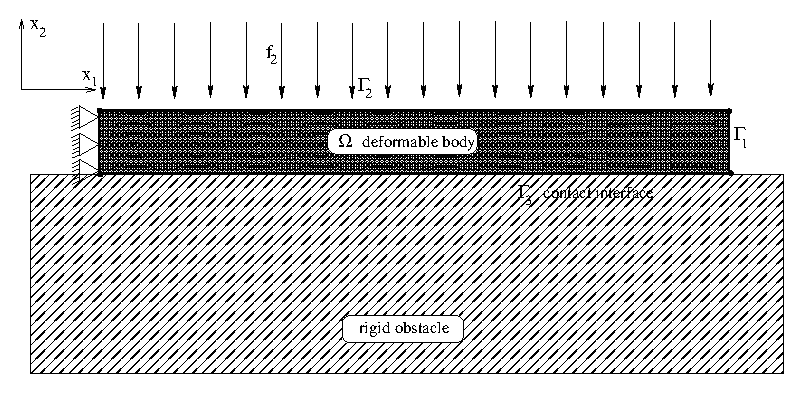
\includegraphics{chapitres/chapitre_2/figures/poutre_conf1.eps}}
	\end{center}
		\caption{Configuration initiale de la poutre contre une fondation.}
		\label{poutre_conf1}
\end{figure}
%ffffffffffffffffffffffffffffff

%ffffffffffffffffffffffffffffff
\begin{figure}[ht!]
	\begin{center}
		 		\resizebox{10cm}{!}{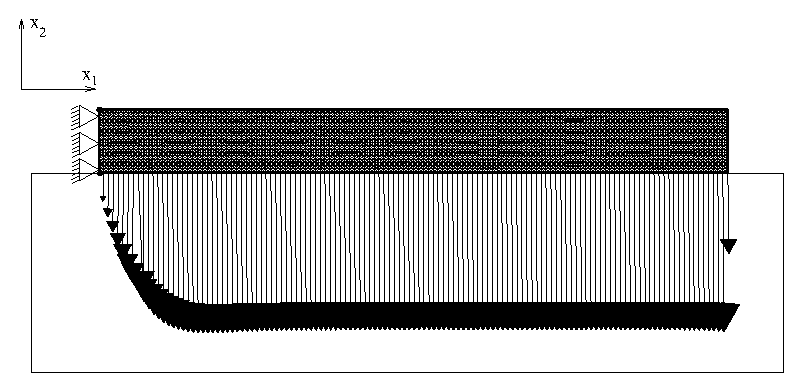
\includegraphics{chapitres/chapitre_2/figures/poutre_def1.eps}}
	\end{center}
		\caption{Configuration déformée de la poutre contre une fondation.}
		\label{poutre_def1}
\end{figure}
%ffffffffffffffffffffffffffffff.
%ffffffffffffffffffffffffffffff
\begin{figure}[ht!]
	\begin{center}
		\resizebox{10cm}{!}{\includegraphics{chapitres/chapitre_2/figures/cont_uniB.eps}}
	\end{center}
	\caption{Contraintes de contact normales sur la zone de contact.}
	\label{cont_uniB}
\end{figure}
%ffffffffffffffffffffffffffffff
%ffffffffffffffffffffffffffffff
\begin{figure}[ht!]
	\begin{center}
		\resizebox{10cm}{!}{\includegraphics{chapitres/chapitre_2/figures/cont_froB.eps}}
	\end{center}
	\caption{Contraintes de frottement tangentielles sur la zone de contact.}
	\label{cont_frotB}
\end{figure}
%ffffffffffffffffffffffffffffff

\noindent\textbf{Précision de la méthode Active Set par rapport à la méthode du quasi-Lagrangien augmenté.}\\

Tout d'abord, nous analysons la précision des contraintes normales et tangentielles de contact avec frottement de la méthode Active Set en la comparant au quasi-Lagrangien augmenté (cf \cite{alart1991mixed}). La frontière $\Gamma_3$ est divisée en 128 parts égales; la contrainte de contact normale $\sigma_{\nu}$ et la contrainte de frottement tangentielle $\|\bsigma_{\tau}\|$ par rapport à l'abscisse sont représentées dans les Figures \ref{cont_uniB} et \ref{cont_frotB} pour chacune des méthodes. Nous noterons que pour $\sigma_{\nu}$ et $\|\bsigma_{\tau}\|$, il n'y a pas de différence visible ($\approx 1\times10^{-7}$), confirmant ainsi la précision sur ce cas de test.\\
Maintenant, nous pouvons comparer l'efficacité des algorithmes mis en oeuvre.\\

\noindent\textbf{Performances des algorithmes}.
Dans la Table \ref{tab1_def}, nous étudions la convergence de la méthode Active Set pour le contact bilatéral associé à la loi de frottement de Tresca en fournissant le nombre de degrés de liberté (ddl), le nombre d'itérations de Newton (Nit) et le temps CPU total en seconde requis pour atteindre la convergence, et ce pour plusieurs valeurs du nombre de noeuds de contact sur la frontière $\Gamma_3$ (nbc). Nous menons la même étude pour la méthode du quasi-Lagrangien augmenté (Table \ref{tab2_def}).
%#######################################################
\begin{table}[htbp!]
\begin{tabular}{ |p{1.25cm}|p{1.25cm}|p{1.25cm}|p{1.25cm}|p{1.25cm}|p{1.25cm}|p{1.25cm}|p{1.25cm}| }
 \hline \rowcolor{lightgray}
 nbc & 8 & 16 & 32 & 64 & 128 & 256 & 512 \\
			\hline
			ddl & 76 & 166 & 586 & 2414 & 10024 & 40528 & 162976 \\
			Nit &  7 & 9 & 9 & 11 & 12 & 13 & 13 \\
			CPU &  $<$1 & $<$1 & $<$1 & 2 & 11 & 70 & 454  \\
 \hline
\end{tabular}
\caption{Résultats de la méthode Active Set pour le contact bilatéral associé à la loi de             frottement de Tresca
	    %(symetric linear systems)
	    en comparaison avec le nombre de degrés de liberté (ddl), le nombre de noeuds de contact (nbc), les itérations de Newton (Nit) et le temps CPU total (CPU) en secondes.}\label{tab1_def}
\end{table}
%#######################################################

%#######################################################
\begin{table}[htbp!]
\begin{tabular}{ |p{1.25cm}|p{1.25cm}|p{1.25cm}|p{1.25cm}|p{1.25cm}|p{1.25cm}|p{1.25cm}|p{1.25cm}| }
 \hline \rowcolor{lightgray}
			nbc & 8 & 16 & 32 & 64 & 128 & 256 & 512 \\
			\hline
			ddl & 92 & 198 & 650 & 2580 & 10280 & 41040 & 164000 \\
			Nit &  5 & 9 & 9 & 11 & 10 & 11 & 9 \\
			CPU &  $<$1 & $<$1 & $<$1 & 5 & 23 & 145 & 807  \\
\hline
\end{tabular}
\caption{Résultats de la méthode du quasi-Lagrangien augmenté pour les lois de contact bilatéral et         de frottement de Tresca
	        %(nonsymetric linear systems)
		     en comparaison avec le nombre de degrés de liberté (ddl), le nombre de noeuds de contact (nbc), les itérations de Newton (Nit) et le temps CPU total (CPU) en secondes.}\label{tab2_def}
\end{table}
%#######################################################
Lorsque $ nbc>64$, la méthode du quasi-Lagrangien augmenté est légèrement plus efficace que la méthode Active Set. Cependant, la méthode Active Set est beaucoup plus rapide en termes de temps CPU que le quasi-Lagrangien, presque deux fois plus rapide. Cela est dû non seulement au fait que la méthode Active Set ne nécessite pas l'utilisation des multiplicateurs de Lagrange mais aussi au fait que la méthode utilise des systèmes linéarisés symétriques, contrairement à la méthode du quasi-Lagrangien augmenté qui présente des sytèmes non-linéarisés symétriques dû au frottement. Cela implique que le système linéaire résultant du problème non-linéaire est plus petit pour la méthode Active Set, comme le confirme la comparaison entre le nombre de degrés de liberté $ddl$ dans les deux cas, et peut être mieux conditionné que le système issu de la méthode du quasi-Lagrangien augmenté, une caractéristique bien connue des problèmes de contact avec frottement.


\subsection{Exemple de contact unilatéral avec frottement de Coulomb}
\label{substatcoulomb}
Dans la configuration $nbc=128$ représentée sur la Figure \ref{poutre_conf2}, 9728 éléments finis élastiques ont été utilisés et le nombre total de degrés de liberté est égal à 10024. Le comportement de l'interaction entre le corps déformable et la fondation est décrit par une loi de contact unilatéral avec la loi de frottement de Coulomb.

Pour le calcul ci-dessous, les données suivantes ont été utilisées:
\begin{eqnarray*}
	\begin{array}{l}
		E= 100N/m^2,\quad \kappa=0.3,\nonumber \\[2mm]
		\fb_0=(0,0) N/m^2, \quad \fb_2= (0,-0.1)\, N/m    \quad \mbox{ sur } 
		\Gamma_2, \nonumber\\[2mm]
		c_\nu=10, \quad c_\tau=10,\quad r_{ lagrangien}=0.1,\quad \mu=0.2, \nonumber\\[2mm]
		{\rm crit\acute{e}re \quad d'arr\hat{e}t}: \epsilon=10^{-6}
	\end{array}
\end{eqnarray*}

Dans la Figure \ref{poutre_def2}, la configuration déformée ainsi que les contraintes de contact normales sur la frontière $\Gamma_3$ sont tracées.\\

%ffffffffffffffffffffffffffffff
\begin{figure}[ht!]
	\begin{center}
		\resizebox{10cm}{!}{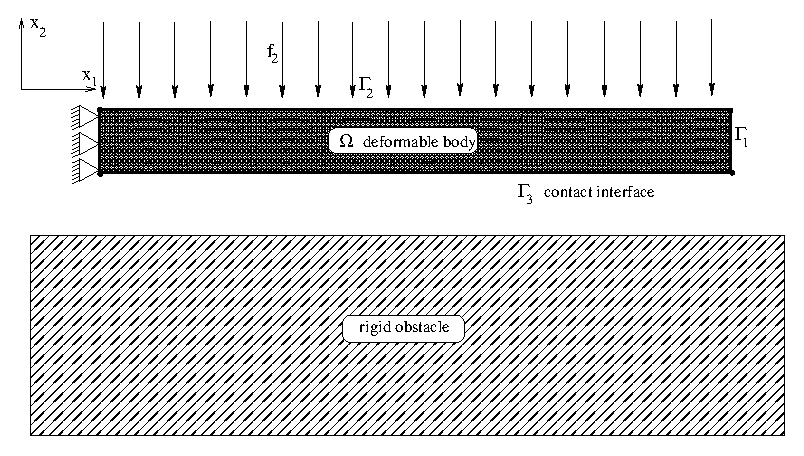
\includegraphics{chapitres/chapitre_2/figures/poutre_conf2.eps}}
	\end{center}
	\caption{Fixation physique de la poutre unilatérale contre une fondation.}
	\label{poutre_conf2}
\end{figure}
%ffffffffffffffffffffffffffffff.

%ffffffffffffffffffffffffffffff
\begin{figure}[ht!]
	\begin{center}
		\resizebox{10cm}{!}{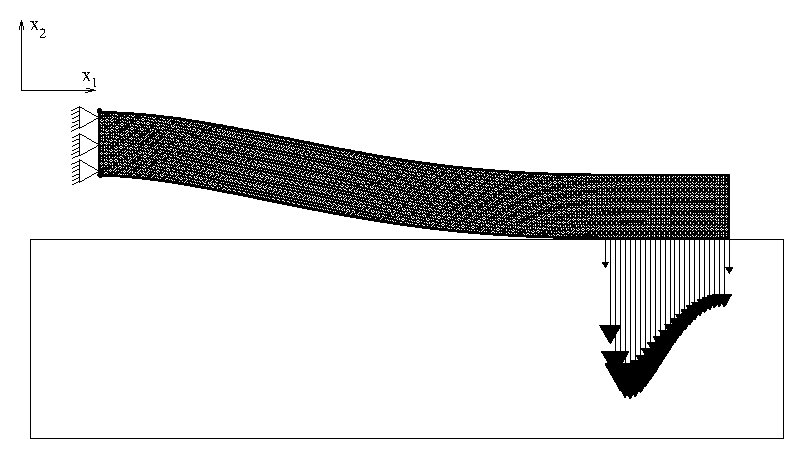
\includegraphics{chapitres/chapitre_2/figures/poutre_def2.eps}}
	 \caption{Configuration déformée de la poutre unilatérale contre une fondation.}
		\label{poutre_def2}
	\end{center}
	
\end{figure}
%ffffffffffffffffffffffffffffff.
\noindent\textbf{Précision de la méthode Active Set par rapport à la méthode du quasi-Lagrangien augmenté.}\\
%ffffffffffffffffffffffffffffff
\begin{figure}[ht!]
	\begin{center}
		\resizebox{10cm}{!}{\includegraphics{chapitres/chapitre_2/figures/cont_uniS.eps}}
	\end{center}
	\caption{Contraintes de contact normales sur la zone de contact.}
	\label{cont_uniS}
\end{figure}
%ffffffffffffffffffffffffffffff
%ffffffffffffffffffffffffffffff
\begin{figure}[ht!]
	\begin{center}
		\resizebox{10cm}{!}{\includegraphics{chapitres/chapitre_2/figures/cont_froS.eps}}
	\end{center}
	\caption{Contraintes de frottement tangentielles sur la zone de contact.}
	\label{cont_frotS}
\end{figure}
%ffffffffffffffffffffffffffffff
Là encore, nous évaluons la précision de la méthode Active Set en la comparant au quasi-Lagrangien augmenté. La frontière $\Gamma_3$ est divisée en 128 parts égales; la contrainte de contact normale $\sigma_{\nu}$ et la contrainte de frottement tangentiel $\|\bsigma_{\tau}\|$ par rapport à l'abscisse sont représentées dans les figures \ref{cont_uniS} et \ref{cont_frotS} pour chacune des méthodes. Encore une fois, il s'avère que pour la contrainte de contact calculée par les deux méthodes, que ce soit $\sigma_{\nu}$ ou $\|\bsigma_{\tau}\|$, il n'y a pas de différence visible ($\approx 1\times10^{-7}$), confirmant ainsi la précision sur ce cas de test.\\

\noindent\textbf{Performances des algorithmes.}\\
Dans la Table \ref{tab3_def}, nous étudions la convergence de la méthode Active Set en fournissant pour le contact unilatéral et la loi de frottement de Coulomb le nombre de degrés de liberté (ddl), le nombre d'itérations de Newton (Nit), le nombre d'itérations de point fixe (fpit) pour approcher la loi de frottement de Coulomb et le temps CPU total (CPU) en seconde requis pour atteindre la convergence, et ce pour plusieurs valeurs du nombre de noeuds de contact sur la frontière $\Gamma_3$ (nbc). Nous menons la même étude pour la méthode du quasi-Lagrangien augmenté pour la loi de contact unilatéral et de frottement de Coulomb (Table \ref{tab4_def}).\\
Dans ce cas, contrairement à la configuration avec contact bilatéral, le nombre d'itérations de Newton n'est plus approprié pour comparer les deux méthodes, car la méthode Active Set approche le frottement de Coulomb avec une boucle interne supplémentaire impliquant une succession d'états de frottement de Tresca tandis que la méthode du quasi-Lagrangien augmenté ne fait pas d'approximation. Par conséquent, le seul critère fiable disponible est le temps CPU. Malgré cette boucle supplémentaire, sur les deux méthodes, la méthode Active Set reste la plus rapide. Lorsque $ nbc = 512 $, l'écart entre les deux méthodes augmente avec le nombre de degrés de liberté. Une telle hypothèse doit être confirmée pour des problèmes plus complexes.\\
%#######################################################
\begin{table}[htbp!]
\begin{tabular}{ |p{1.25cm}|p{1.25cm}|p{1.25cm}|p{1.25cm}|p{1.25cm}|p{1.25cm}|p{1.25cm}|p{1.25cm}| }
 \hline \rowcolor{lightgray}
			nbc & 8 & 16 & 32 & 64 & 128 & 256 & 512 \\
			\hline
			ddl & 76 & 166 & 586 & 2414 & 10024 & 40528 & 162976 \\
			Nit &  15 & 25 & 37 & 45 & 44 & 46 & 39 \\
            fpit &  5 & 5 & 5 & 5 & 5 & 5 & 7 \\
			CPU &  $<$1 & $<$1 & 1 & 9 & 61 & 364 & 1448  \\
\hline
\end{tabular}
\caption{Résultats de la méthode Active Set pour les lois de contact unilatéral et de               frottement de Tresca %(fixed point method - symetric linear systems)
		   en comparaison avec le nombre de degrés de liberté (ddl), le nombre de noeuds de contact (nbc), les itérations de Newton (Nit), les itérations de point fixe (fpit) et le temps CPU total (CPU) en secondes.}\label{tab3_def}
\end{table}
%#######################################################

%#######################################################
\begin{table}[htbp!]
\begin{tabular}{ |p{1.25cm}|p{1.25cm}|p{1.25cm}|p{1.25cm}|p{1.25cm}|p{1.25cm}|p{1.25cm}|p{1.25cm}| }
 \hline \rowcolor{lightgray}
			nbc & 8 & 16 & 32 & 64 & 128 & 256 & 512 \\
			\hline
			ddl & 92 & 198 & 650 & 2580 & 10280 & 41040 & 164000 \\
			Nit &  4 & 17 & 20 & 23 & 26 & 27 & 28 \\
			CPU &  $<$1 & $<$1 & 1 & 9 & 62 & 405 & 2972  \\
\hline
\end{tabular}
	\caption{Résultats de la méthode du quasi-Lagrangien augmenté pour les lois de contact unilatéral et de frottement de Coulomb en comparaison avec le nombre de degrés de liberté (ddl), le nombre de nœuds de contact (nbc), les itérations de Newton (Nit) et le temps CPU total (CPU) en secondes.} \label{tab4_def}
\end{table}
%#######################################################

\section{Simulations numériques dans le cas dynamique}\label{simu_dynam}

Après avoir évalué les performances et la précision des méthodes Active Set implémentées sur des cas statiques simples, notre objectif désormais est d'évaluer la robustesse de ces méthodes sur des problèmes plus complexes. Les simulations dans cette partie sont réalisées à partir de deux configurations de contact dynamique: le contact unilatéral avec la loi de frottement de Coulomb d'une poutre élastique linéaire sur une fondation rigide, puis le rebond d'un anneau hyper-élastique contre une fondation rigide. La solution numérique du problème ${\cal P}$ est calculée par les méthodes Active Set et quasi-Lagrangien augmenté afin de mettre en évidence les performances de la première méthode par rapport à la seconde.
Comme pour les exemples numériques de la section précédente, le domaine $\Omega$ représente la section transversale d'un corps déformable tridimensionnel soumis à l'action de la vitesse initiale de telle sorte qu'une hypothèse de contrainte plane est supposée.


\subsection{Exemple académique: compression d'une poutre contre une fondation rigide}

La configuration de référence est la même que celle introduite dans la sous-section \ref{substatcoulomb}.

Pour le calcul ci-dessous, les données suivantes ont été utilisées:
\begin{eqnarray*}
	\begin{array}{l}
		\rho = 1000kg/m^3, \quad T=0.5s,  \quad k=\frac{1}{10}, \nonumber \\[2mm]
		E= 10N/m^2,\quad \kappa=0.3,\nonumber \\[2mm]
		\fb_0=(0,0) N/m^2, \quad \fb_2= (0,-0.1)\, N/m    \quad \mbox{ sur }
		\Gamma_2, \nonumber\\[2mm]
		c_\nu=10, \quad c_\tau=10,\quad r_{lagrangien}=0.1\nonumber, \quad \mu = 0.2\\[2mm]
		{\rm crit\acute{e}re \quad d'arr\hat{e}t}: \epsilon=10^{-6}.
	\end{array}
\end{eqnarray*}

\noindent\textbf{Précision de la méthode Active Set par rapport à la méthode du quasi-Lagrangien augmenté dans le cas dynamique.}\\
Nous allons à présent évaluer la précision de la méthode Active Set en la comparant au quasi-Lagrangien augmenté dans le cas dynamique. La frontière  $\Gamma_3$ est divisée en $128$ parts égales; la contrainte de contact normale $\sigma_{\nu}$ et la contrainte de frottement tangentiel $\|\bsigma_{\tau}\|$ par rapport à l'abscisse sont représentées dans les Figures \ref{cont_uniD} et \ref{cont_froD} pour chacune des méthodes. Nous constatons ainsi qu'il n'y a aucune différence entre la contrainte de contact calculée par les deux méthodes.\\

%%ffffffffffffffffffffffffffffff

\begin{figure}[ht!]
            \begin{center}
                   \resizebox{10cm}{!}{\includegraphics{chapitres/chapitre_2/figures/cont_uniD.eps}}
            \end{center}
            \caption{Contraintes de contact normales sur la zone de contact.}
            \label{cont_uniD}
\end{figure}

%%ffffffffffffffffffffffffffffff
%%ffffffffffffffffffffffffffffff

\begin{figure}[ht!]
            \begin{center}
                      \resizebox{10cm}{!}{\includegraphics{chapitres/chapitre_2/figures/cont_froD.eps}}
            \end{center}
            \caption{Contraintes de frottement tangentielles sur la zone de contact.}
            \label{cont_froD}
\end{figure}
%%ffffffffffffffffffffffffffffff

\noindent\textbf{Performances des algorithmes.}\\
Pour cet exemple, la méthode Active Set fonctionne mieux que la méthode du quasi-Lagrangien augmenté uniquement lorsque $ nbc> 512 $ (voir Table \ref{tab5_def} et \ref{tab6_def}). Cependant, d'après la Figure \ref{dynaelas_CPU}, plus le nombre de noeuds de contact est grand, plus l'écart de temps CPU entre les méthodes croît, rendant ainsi la méthode Active Set plus pertinente.

%#######################################################
\begin{table}[htbp!]
\begin{tabular}{ |p{1.25cm}|p{1.25cm}|p{1.25cm}|p{1.25cm}|p{1.25cm}|p{1.25cm}|p{1.25cm}|p{1.25cm}| }
 \hline \rowcolor{lightgray}
			nbc & 8 & 16 & 32 & 64 & 128 & 256 & 512 \\
			\hline
			ddl & 76 & 166 & 586 & 2414 & 10024 & 40528 & 162976 \\
			Ntit &  119 & 153 & 191 & 254 & 258 & 240 & 216 \\
			afpit &  4 & 4 & 4 & 4 & 5 & 4 & 5 \\
			CPU &  0.07 & 0.33 & 2.52 & 25.57 & 162.28 & 861.92 & 3295.57  \\
\hline
\end{tabular}
	\caption{Résultats de la méthode Active Set pour le contact unilatéral et frottement de Coulomb en comparaison avec le nombre de degrés de liberté (ddl), le nombre de noeuds de contact (nbc), le nombre total d'itérations de Newton (Ntit), de point fixe moyen (afpit) et le temps CPU total (CPU) en secondes.} \label{tab5_def}
\end{table}
%#######################################################

%#######################################################
\begin{table}[htbp!]
\begin{tabular}{ |p{1.25cm}|p{1.25cm}|p{1.25cm}|p{1.25cm}|p{1.25cm}|p{1.25cm}|p{1.25cm}|p{1.25cm}| }
 \hline \rowcolor{lightgray}
			nbc & 8 & 16 & 32 & 64 & 128 & 256 & 512 \\
			\hline
			ddl & 92 & 198 & 650 & 2580 & 10280 & 41040 & 164000 \\
			Ntit &  37 & 58 & 80 & 87 & 98 & 112 & 119 \\
			CPU &  0.04 & 0.28 & 2.25 & 20.05 & 113.78 & 769.38 & 5773.57  \\
\hline
\end{tabular}
	\caption{Résultats de la méthode du quasi-Lagrangien augmenté pour le contact unilatéral et frottement de Coulomb en comparaison avec le nombre de degrés de liberté (ddl), le nombre de nœuds de contact (nbc), le nombre total d'itérations de Newton (Ntit) et le temps CPU total (CPU) en secondes.} \label{tab6_def}
\end{table}
%#######################################################

\begin{figure}[ht!]
	\begin{center}
		\resizebox{10cm}{!}{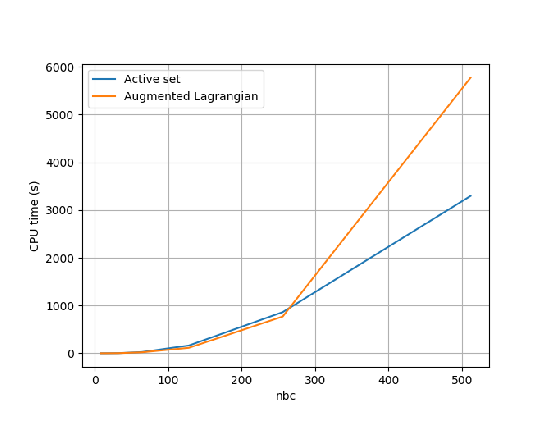
\includegraphics{chapitres/chapitre_2/figures/dynaelas}}
	\end{center}
	\caption{Temps CPU pour les méthodes Active Set et quasi-Lagrangien augmenté en fonction de $ nbc $.}
	\label{dynaelas_CPU}
\end{figure}
%ffffffffffffffffffffffffffffff

\subsection{Exemple pertinent: rebond d'un anneau hyper-élastique contre une fondation rigide}
%ffffffffffffffffffffffffffffff
\begin{figure}[!h]
	\begin{center}
			\resizebox{10cm}{!}{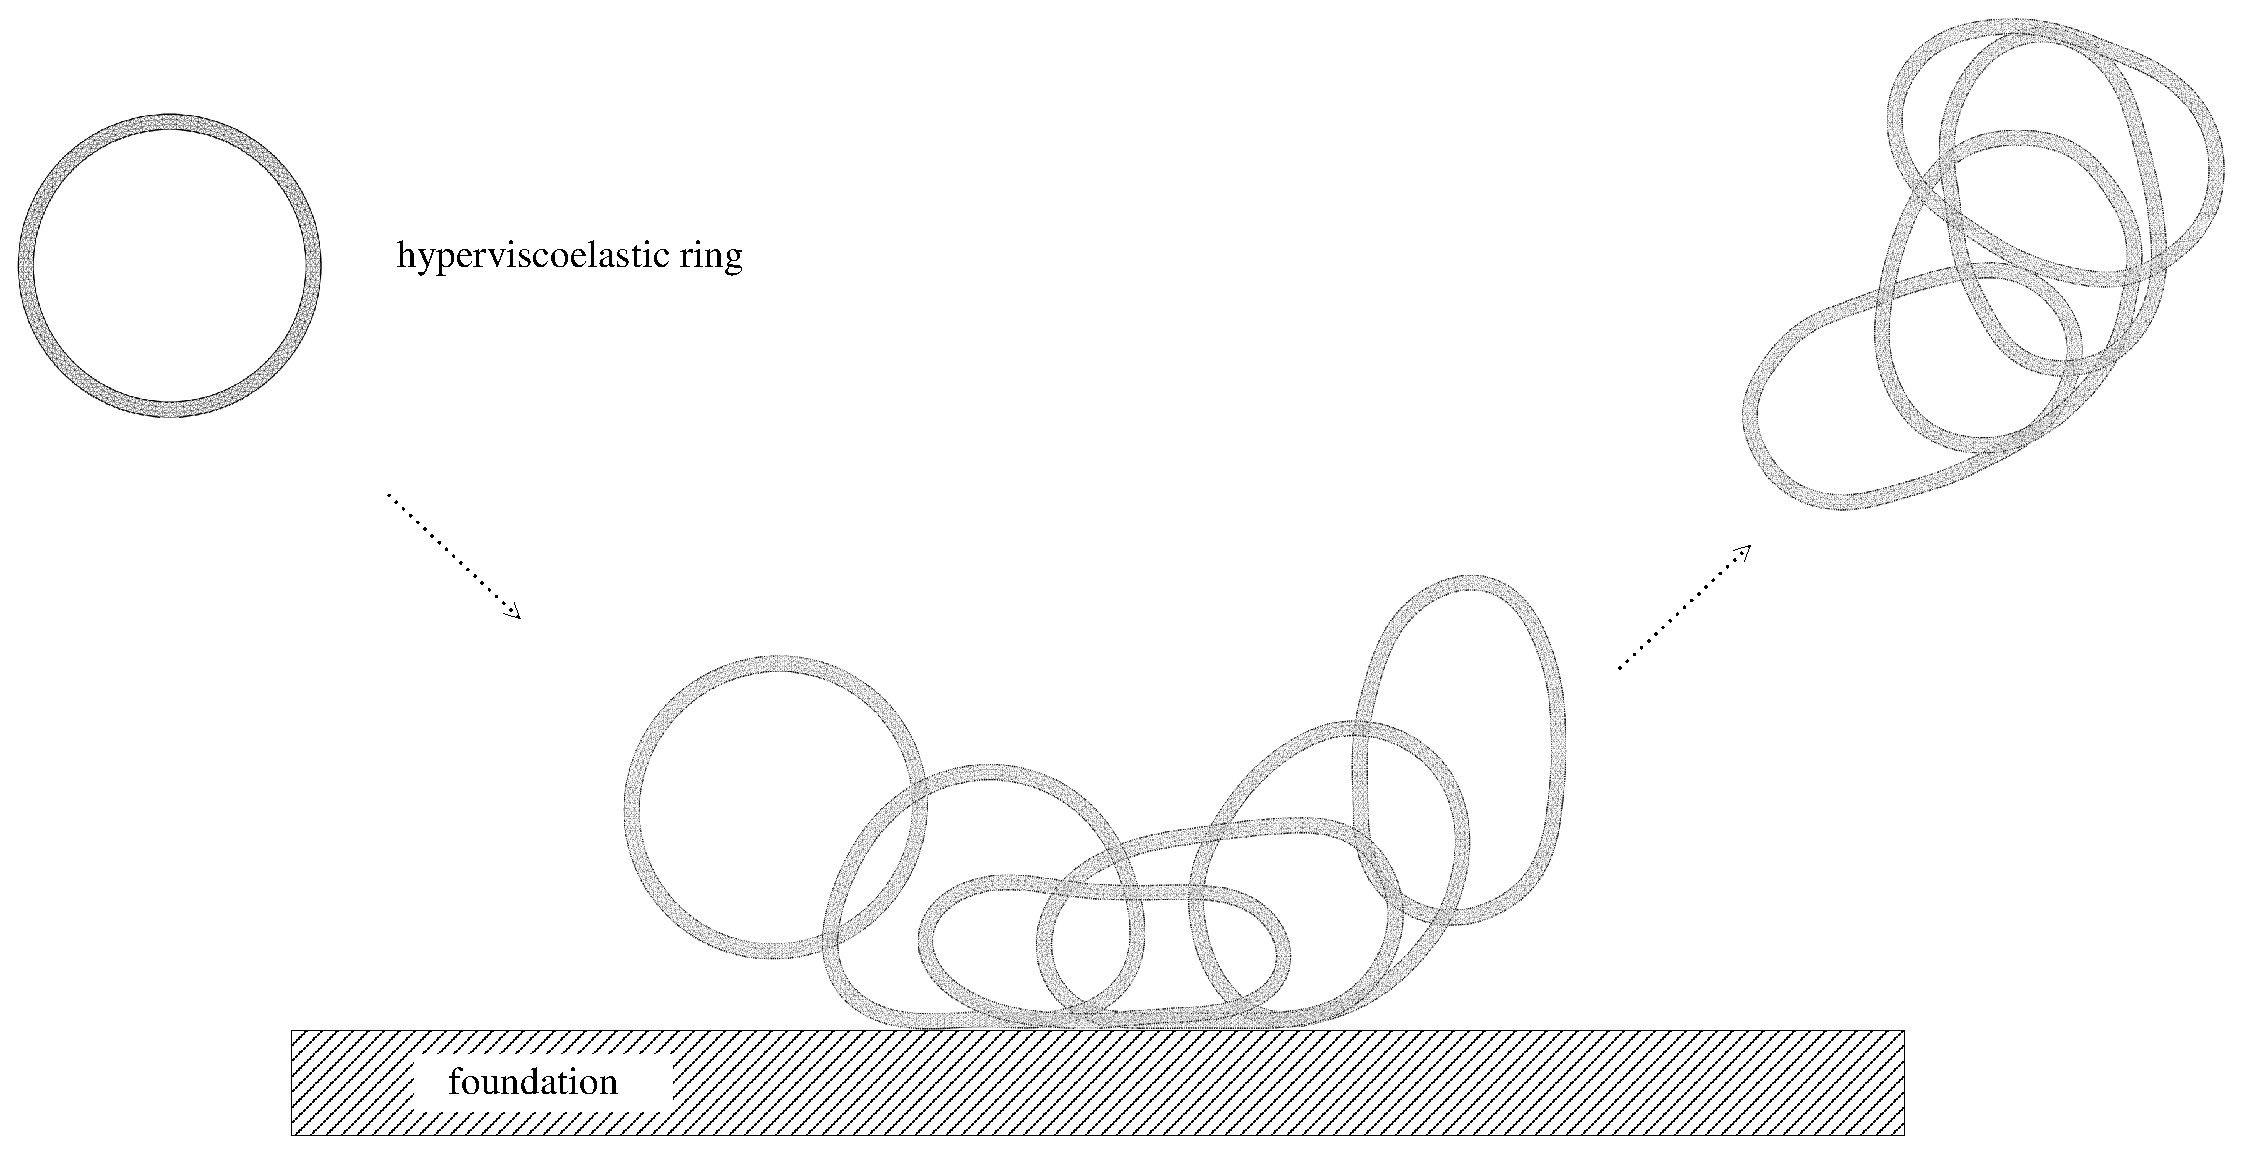
\includegraphics{chapitres/chapitre_2/figures/ring_sequence}}
	\end{center}
	\caption{Séquence de l'anneau hyper-élastique déformé avant, pendant et après l'impact.}
	\label{ring_test}
\end{figure}
%ffffffffffffffffffffffffffffff
Nous considérons maintenant une deuxième application représentative afin d'évaluer les performances des méthodes types Active Set dans le cas d'un cadre en grandes déformations. Il s'agit d'un exemple plus pertinent que les exemples précédents de problème de contact avec frottement.\\
Pour la discrétisation, nous choisissons un paramètre $ nbc $ décrivant le nombre de nœuds de contact sur $ \Gamma $ (le nombre de noeuds sur le contour extérieur de l'anneau est donc pris afin d'obtenir des éléments suffisamment réguliers) . Dans la configuration $ nbc = 128 $ représentée sur la Figure \ref{ring_test}, la frontière $\Gamma_3$ est divisée en 128 parts égales, 1664 éléments finis hyper-élastiques ont été utilisés pour un nombre total de degrés de liberté égal à 2048.
La réponse du matériau compressible, considérée ici, est régie par une variante de la loi de comportement d'Ogden (cf \cite{ciarlet1982lois}) définie par la densité d'énergie suivante


%
%%%%%%%%%%%%%%%%%%%%%%%%%
\begin{equation}\nonumber
W({\bf C}) = c_1 (I_1 - 3) + c_2 (I_2 - 3) + a (I_3 - 1) - (c_1 + 2 c_2 + a) \ln
I_3.
\end{equation}
%%%%%%%%%%%%%%%%%%%%%%%%%%%%%
\noindent Ici $I_1, I_2$ et $I_3 $ représentent les trois invariants
du tenseur de Cauchy ${\bf C}$, avec ${\bf C} = {\bf F}^{\bf T} {\bf F}$. 

Les détails sur la configuration physique du problème sont donnés ci-dessous. Le domaine $ \Omega $ est défini par:
\begin{align*}
\Omega\, &=\left\{(x_1,x_2)\in \mathbb{R}^2:  \ 81 <(x_1-100)^2
+ (x_2-100)^2 \leq 100 \right\},\\
\Gamma_1&=  \varnothing, \qquad \Gamma_2=  \varnothing,\\
\Gamma_3&=\left\{(x_1,x_2)\in \mathbb{R}^2: \ (x_1-100)^2
+ (x_2-100)^2 = 100 \right\}.
\end{align*}

Le domaine $ \Omega $ représente la section d'un corps déformable tridimensionnel sous l'hypothèse de contrainte plane. L'anneau est projeté avec une vitesse initiale à un angle de $45^o$ vers une fondation comme le montre la Figure \ref{ring_test}. La fondation est donnée par $\left\{(x_1,x_2)\in \mathbb{R}^2:  \ x_2 \leq 0  \right\}$. Pour la discrétisation, nous utilisons 1664 noeuds élastiques et 128 noeuds de contact. Pour les expériences numériques, les données sont:
\begin{eqnarray}
\begin{array}{l}
\rho = 1000 kg/m^3, \quad T=5s,  \quad k=\frac{1}{500}, \nonumber \\[2mm]
\bu_0=(0,0) m,  \quad \bu_1=(10,-10) m/s, \nonumber \\[2mm]
c_1 = 0.5 MPa, \quad c_2 = 0.05 MPa, \quad a = 0.5x10^{-4} MPa,  \nonumber \\[2mm]
c_\nu=10, \quad c_\tau=10,\quad r_{lagrangien}=0.1\nonumber\\[2mm]
g=50\,m,  \quad \mu = 0.2, \nonumber \\[2mm]
{\rm crit\acute{e}re \quad d'arr\hat{e}t}: \epsilon=10^{-6}.
\end{array}
\end{eqnarray}

Comme dans la section précédente, nous comparons les résultats obtenus par la méthode Active Set et la méthode du quasi-Lagrangien augmenté en ce qui concerne la convergence et les performances des méthodes (voir Tables \ref{tab7_def} et \ref{tab8_def}). 
%#######################################################
\begin{table}[htbp!]
\begin{tabular}{ |p{1.8cm}|p{1.8cm}|p{1.8cm}|p{1.8cm}|p{1.8cm}|p{1.8cm}| }
 \hline \rowcolor{lightgray}
			nbc  & 32 & 64 & 128 & 256 & 512 \\
			\hline
			ddl & 192 & 384 & 1792 & 4608 & 15360  \\
			Ntit &  1876 & 1904 & 1944 & 1961 & 2022  \\
			afpit &  4 & 4 & 4 & 4 & 4  \\
			CPU &  6.32 & 12.39 & 99.22 & 304.62 & 1841.23   \\
\hline
\end{tabular}
	\caption{Résultats de la méthode Active Set pour les lois de contact unilatéral et de frottement de Coulomb en comparaison avec le nombre de degrés de liberté (ddl), le nombre de noeuds de contact (nbc), le nombre total d'itérations de Newton (Ntit), de point fixe moyen (afpit) et le temps CPU total (CPU) en secondes.} \label{tab7_def}
\end{table}
%#######################################################

%#######################################################
\begin{table}[htbp!]
\begin{tabular}{ |p{1.8cm}|p{1.8cm}|p{1.8cm}|p{1.8cm}|p{1.8cm}|p{1.8cm}| }
 \hline \rowcolor{lightgray}
			nbc  & 32 & 64 & 128 & 256 & 512 \\
			\hline
			ddl & 256 & 512 & 2048 & 5120 & 16384  \\
			Ntit &  1462 & 1568 & 1705 & 1782 & 1866  \\
			CPU &  8.59 & 18.03 & 139.69 & 428.80 & 2693.86   \\
\hline
\end{tabular}
	\caption{Résultats de la méthode du quasi-Lagrangien augmenté pour les lois de contact unilatéral et de frottement de Coulomb en comparaison avec le nombre de degrés de liberté (ddl), le nombre de nœuds de contact (nbc), le nombre total d'itérations de Newton (Ntit) et le temps CPU total (CPU) en quelques secondes.} \label{tab8_def}
\end{table}
%#######################################################

Bien que ce cas soit assez complexe, les performances de la méthode Active Set s'améliorent. D'après la Figure \ref{dynahyper_CPU}, plus le nombre de noeuds de contact est grand, plus l'écart de temps CPU entre les méthodes s'élargit, ce qui est cohérent avec notre hypothèse de la partie précédente, et confirme la robustesse de ces méthodes sur des configurations complexes. Cependant, cela ne suffit pas pour expliquer le gain en temps CPU de la méthode Active Set approchée par rapport à la méthode du quasi-Lagrangien augmenté. Comme mentionné à la fin de la section \ref{fullcoulombactive}, les systèmes linéarisés sont symétriques, même en cas de frottement, alors qu'ils ne le sont pas pour le quasi-Lagrangien. Ainsi, la symétrie des systèmes linéarisés et l'absence des multiplicateurs de Lagrange sont des arguments pertinents et solides en faveur des méthodes types Active Set. 

\begin{figure}[h!]
	\begin{center}
		\resizebox{10cm}{!}{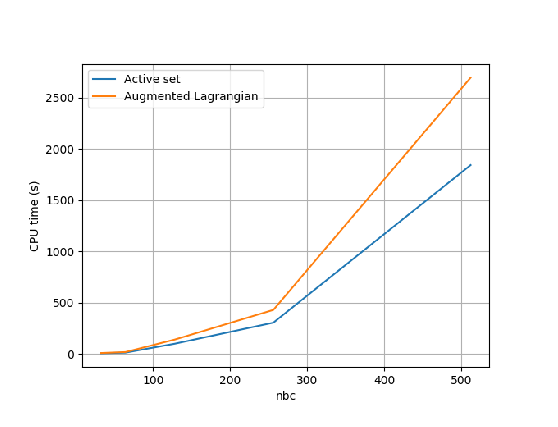
\includegraphics{chapitres/chapitre_2/figures/dynahyper.eps}}
	\end{center}
	\caption{Temps CPU pour la méthode Active Set et le quasi-Lagrangien augmenté en fonction de $nbc$.}
	\label{dynahyper_CPU}
\end{figure}
%ffffffffffffffffffffffffffffff

Cet exemple montre clairement la robustesse de la méthode Active Set dans une configuration complexe. Il semble que l'absence des multiplicateurs de Lagrange reste un argument solide pour choisir la méthode Active Set plutôt que la méthode du quasi-Lagrangien augmenté pour la résolution numérique de ce genre de problèmes de contact.




 
\section{Compléments des méthodes de type Active Set sur les conditions de contact persistant}\label{complement_persistant}

Nous présentons dans cette section quelques compléments numériques sur les méthodes de type Active Set dans le cadre d'un contact persistant. D'ailleurs, cette partie servira de transition avec le chapitre suivant car une telle loi permet de conserver l'énergie durant le contact. Pour illustrer cela, nous considérons le cas d'une balle élastique linéaire qui rebondit sur une fondation rigide pour laquelle nous étudions la séquence de déformation au cours du temps ainsi que les forces de contacts qui s'y exercent dessus avant, pendant et après l'impact.  

\subsection{Conditions de contact persistants}\label{cont_cond}

Lorsqu'un contact ponctuel a lieu entre une balle élastique linéaire (solide déformable) et une fondation rigide, une force de répulsion normale qui vérifie les conditions de Signorini est exercée au point de contact. L'énergie fournie par cette force est alors conservée (voir \cite{laursen2013computational}, \cite{laursen1997design}) sous réserve qu'une condition de persistence (\ref{pers_not_gap_2}) s'ajoute aux conditions de contact unilatéral (\ref{pers_gap})--(\ref{pers_not_gap_1}). Cette condition signifie qu'il ne peut y avoir d'impulsion normale de contact que lorsque celle-ci est persistente. Par ailleurs, si un frottement sec est pris en compte, il introduit une relation entre l'impulsion de contact et la vitesse relative locale de la balle élastique. Les conditions de contact et de frottement sont alors basées sur la combinaison des conditions de contact unilatéral  exprimées en vitesse avec une loi de Coulomb de frottement sec. L'ajout de la condition de persistence aux conditions de contact unilatéral (voir preuve dans \cite{laursen2013computational}, \cite{moreau1994numerical} et \cite{moreau1999sweeping}) permet d'écrire:

\begin{eqnarray}  
&\mbox{si} \ \ d_{\nu} > 0  \quad & \lambda_{\nu} = 0 \ ;\ \blambda_{\tau} =0  \label{pers_gap} \\
&\mbox{si} \ \ d_{\nu} = 0  \quad & \\ 
&&\dot u_{\nu} \ge 0 \label{pers_not_gap},\\
&&\lambda_{\nu}\ge 0 \label{pers_not_gap_1},\\
&&\dot u_{\nu}\lambda_{\nu}= 0 \label{pers_not_gap_2},\\
&& \left\{\begin{array}{ll} \label{pers_not_gap_coulomb}
\|\blambda_{\tau}\|\le\,\mu |\lambda_{\nu}|,\\[2mm]
\|\blambda_{\tau}\|<\,\mu |\lambda_{\nu}|\Longrightarrow \dot\bu_{\tau}=0,\\[2mm]
\|\blambda_{\tau}\|=\,\mu |\lambda_{\nu}|\Longrightarrow \exists \beta\ge 0: \blambda_{\tau}=\beta \dot\bu_{\tau}, \end{array}\right .
 \end{eqnarray}
 
$g$ étant la distance minimale autorisée (interstice) entre un point de la surface de contact et sa projection sur la fondation rigide. La loi de frottement de Coulomb (\ref{pers_not_gap_coulomb}) dépend de la contrainte de  frottement  tangentielle $\blambda_{\tau}$,  de  la  pression  de  contact  normale  $\lambda_{\nu}$ et de la  vitesse  de  contact tangentielle $\dot\bu_{\tau}$.

\subsection{Méthode de type "Primal-dual Active Set"}\label{Activeset_type}

Les conditions de contact unilatéral avec frottement dans le cadre d'un contact persistant (\ref{pers_gap})--(\ref{pers_not_gap_coulomb}) sont réalisées en appliquant une stratégie Active Set sur les fonctions de complémentarité non-linéaires ${\cal R}_{\nu}^{\blambda}$ et ${\cal R}_{\tau}^{\blambda}$ basées sur un formalisme itératif de Newton semi-régulier. Les ensembles actifs et inactifs sont définis selon un schéma de point milieu "\textit{leapfrog}" défini comme suit:

\begin{align*}
&d_{\nu}^{leapfrog} = d_{\nu,p} + \frac{\Delta{t}}{2} \dot u_{\nu,p},
\end{align*}

\noindent avec $\dot u_{\nu,p} = \frac{u_{\nu,p}-u_{\nu,p-1}}{\Delta{t}}$. Le statut d'un noeud donné à l'itération $k$ dépend de l'ensemble auquel il appartient; sur la base des parties précédentes, il peut être à l'état sans contact, avec contact glissant ou avec contact adhérant.\\

\noindent La description de l'algorithme itératif Active Set d'indice $k$ dans le cadre d'un contact persistant est la suivante:\\

\noindent (i) \quad Choisir $(\bu^{(0)},\blambda^{(0)})$, $c_{\nu}>0$, $c_\tau>0$ et initialiser $k=0$.\\[3mm]
\qquad(ii) \quad si \ $d_{\nu}^{leapfrog} > 0$ \qquad  $\lambda^{(k)}_{\nu,p} = 0$ \ ;\ $\blambda_{\tau, p}^{(k)} =0$ \\[3mm]
\qquad(iii) \quad si \ $d_{\nu}^{leapfrog} \le 0$  \qquad les ensembles actifs et inactifs:
\begin{align*}
&{\cal A}_{\nu}^{k+1}=\{p\in {\cal S}:\lambda^{(k)}_{\nu,p}+c_{\nu} \dot u^{(k)}_{\nu,p}> 0\},\\
&{\cal I}_{\nu}^{k+1}={\cal S}\setminus {\cal A}_{\nu}^{k+1},\\
&{\cal A}_{\tau}^{k+1}=\{p\in {\cal S}:\|\blambda_{\tau, p}^{(k)}+c_\tau \dot\bu_{\tau, p}^{(k)}\|-\mu \lambda_{\nu, p}^{(k)}> 0\},\\
&{\cal I}_{\tau}^{k+1}={\cal S}\setminus {\cal A}_{\tau}^{k+1}.
\end{align*}
(iv) Trouver $(\bu^{(k+1) },\blambda^{(k+1) })$ tel que
\begin{eqnarray}
& \rho \ddot{\bu}^{(k+1)}+ A(\bu^{(k+1)}) + \lambda_{\nu}^{(k+1)}\nu + \blambda_{\tau}^{(k+1)}= \fb, \\[1mm]
&\label{Anu}\dot u^{(k+1)}_{\nu,p}=0 \quad {\rm pour \ tout} \quad p\in {\cal A}_{\nu}^{k+1},\\[1mm]
&\label{Inu}\lambda^{(k+1)}_{\nu,p}=0, \quad \blambda^{(k+1)}_{\tau,p}=\bzero \quad {\rm pour \ tout} \quad p\in {\cal I}_{\nu}^{k+1},\\[1mm]
&\label{Atau}\blambda_{\tau, p}^{(k+1)} = \mu \lambda_{\nu, p}^{(k+1)} \frac{\blambda_{\tau, p}^{(k)}+c_\tau \dot\bu_{\tau, p}^{(k)}}{\|\blambda_{\tau, p}^{(k)}+c_\tau \dot\bu_{\tau, p}^{(k)}\|} \quad {\rm pour \ tout} \ p\in {\cal A}_{\tau}^{k+1}\cap {\cal A}_{\nu}^{k+1},\\[1mm]
&\label{Itau}\dot\bu_{\tau, p}^{(k+1)}+\frac{\dot\bu_{\tau, p}^{(k)}}{\lambda_{\nu, p}^{(k)}}\lambda_{\nu, p}^{(k+1)} =\dot\bu_{\tau, p}^{(k)} \quad {\rm pour \ tout} \ p\in {\cal I}_{\tau}^{k+1}\cap {\cal A}_{\nu}^{k+1}.
\end{eqnarray}
(v) Si $\|(\bu^{(k+1) },\blambda^{(k+1)})-(\bu^{(k) },\blambda^{(k)})\|\leq\epsilon$, $\|{\cal R}(\bu^{(k+1) },\blambda^{(k+1)})\|\leq\epsilon$, ${\cal A}_{\nu}^{k+1}={\cal A}_{\nu}^{k}$ et ${\cal A}_{\tau}^{k+1}={\cal A}_{\tau}^{k}$ alors stop, sinon retourner à (ii).\\[1mm]

\subsection{Impact d'une balle élastique linéaire contre une fondation} \label{num_ex1}
Ce problème de référence représentatif décrit l'impact sans frottement d'une balle élastique linéaire contre une fondation (voir \cite{khenous2006discretization}). 
La balle élastique est lancée avec une vitesse initiale ($\bu_1=(0,-10) m/s$) vers la fondation\\
$\left\{(x_1,x_2)\in \mathbb{R}^2:  \ x_2 \leq 0 \right\}$. Le comportement du matériau est décrit par une loi de comportement linéaire élastique définie par la densité d'énergie:

\begin{equation}
	W^e(\bvarepsilon)=\frac{E\kappa}{2(1+\kappa)(1-2\kappa)} (tr
	\bvarepsilon)^2 +\frac{E}{2(1+\kappa)} tr(\bvarepsilon^2), \quad \forall
	\epsilon \in \mathbb{M}^n.
\end{equation}

Ici, $E$ et $\kappa$ sont le module de Young et le rapport de Poisson du matériau et $tr(\cdot)$ désigne la fonction trace, respectivement. Notez que $\bvarepsilon = \frac{1}{2} ({\nabla \bu}^T + \nabla \bu)$ représente le tenseur de déformation linéarisé dans le cadre de la théorie des petites déformations ($\|\bu\|<< 1$ et $\|\nabla \bu\| << 1$ dans $\Omega$).

%%%%%%%%%%%%%%%%%%%%%%%%%%%%%%%%%%%%%%%%%%%%%%%%%%%%%%%%%%%%%%%%%%%%%%%%%%%%%%
\begin{figure}[!h]
	\begin{center}
		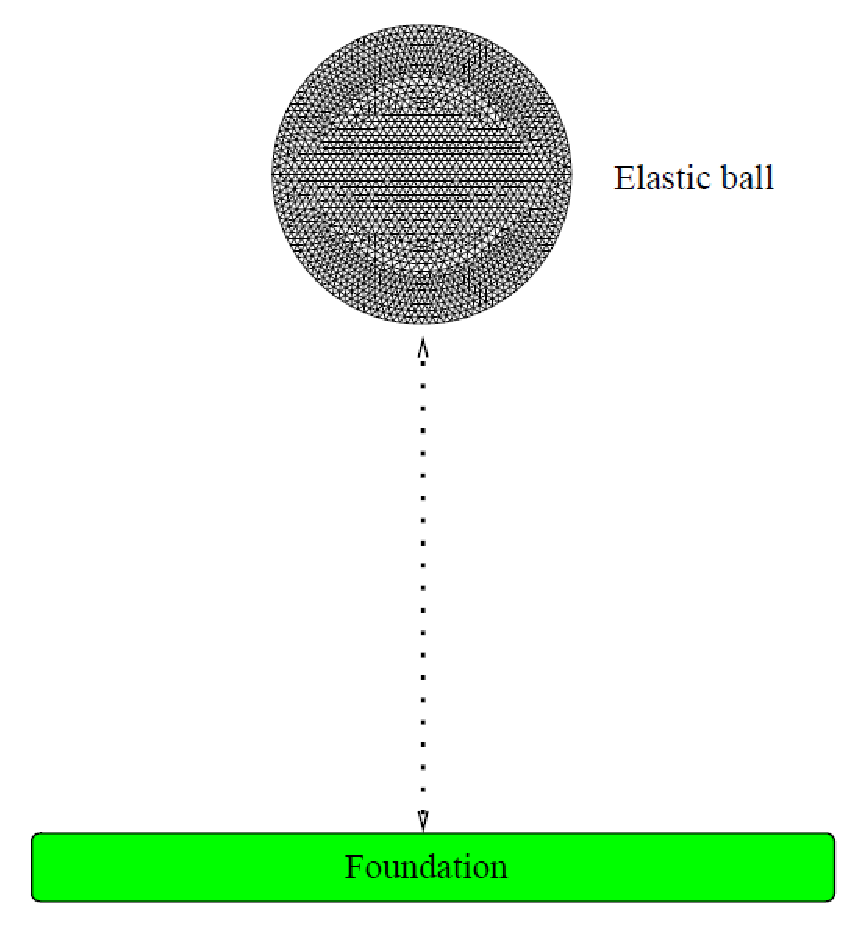
\includegraphics[width=6cm]{chapitres/chapitre_2/figures/ex_num.eps}
	\end{center}
	\caption{Discrétisation de la balle élastique au contact d'une fondation.}
	\label{fig_num1}
\end{figure}
%%%%%%%%%%%%%%%%%%%%%%%%%%%%%%%%%%%%%%%%%%%%%%%%%%%%%%%%%%%%%%%%%%%%%%%%%%%%%%
Le cadre physique est illustré dans la Figure \ref{fig_num1}.
\begin{align*}
\Omega\, &=\left\{(x_1,x_2)\in \mathbb{R}^2:  \ (x_1-100)^2
+ (x_2-100)^2 \leq 100 \right\},\\
\Gamma_1&=  \varnothing, \qquad \Gamma_2=  \varnothing,\\
\Gamma_3&=\left\{(x_1,x_2)\in \mathbb{R}^2: \ (x_1-100)^2
+ (x_2-100)^2 = 100 \right\}.
\end{align*}
Le domaine $\Omega$ représente la section transversale de la balle, sous l'hypothèse de la contrainte plane. Aucune force volumique n'est supposée agir sur le corps pendant le processus. Pour la discrétisation du problème de contact représenté, nous utilisons 7820 noeuds élastiques et 128 noeuds multiplicateurs de Lagrange. Pour les expériences numériques, nous utilisons les données suivantes:
\begin{eqnarray}
\begin{array}{l}
\rho = 1000 kg/m^3, \quad T=2s,  \quad k=0.001, \nonumber \\[2mm]
\bu_0=(0,0) m,  \quad \bu_1=(0,-10) m/s, \nonumber \\[2mm]
E= 100 GPa,\quad \kappa=0.35, \quad \fb_0=(0,0) Pa,  \nonumber \\[2mm]
g=50\,m, \quad c_{\nu} = c_{\tau} = 10, \quad \mu = 0. \nonumber
\end{array}
\end{eqnarray}
%%%%%%%%%%%%%%%%%%%%%%%%%%%%%%%%%%%%%%%%%%%%%%%%%%%%%%%%%%%%%%%%%%%%%%%%%%%%%%

Dans la Figure \ref{defcont}, la séquence de la balle déformée
ainsi que les forces de contact sont présentées avant, pendant et
après l'impact.\\
%%%%%%%%%%%%%%%%%%%%%%%%%%%%%%%%%%%%%%%%%%%%%%%%%%%%%%%%%%%%%%%%%%%%%%%%%%%%%%
\begin{figure}[!h]
	\begin{center}
		\includegraphics[width=11.5cm]{chapitres/chapitre_2/figures/def.eps}
	\end{center}
	\caption{Séquence de la balle déformée et des forces de contact avant, pendant et après l'impact.}\label{defcont}
\end{figure}
%%%%%%%%%%%%%%%%%%%%%%%%%%%%%%%%%%%%%%%%%%%%%%%%%%%%%%%%%%%%%%%%%%%%%%%%%%%%%%
L'intérêt de cet exemple représentatif est de comparer les résultats numériques de la méthode Active-Set obtenus en utilisant certaines méthodes classiques. À cette fin, nous considérons cinq méthodes existantes: 
\begin{itemize}
    \item La méthode quasi-Lagrangien augmenté classique avec condition de contact de Signorini ($r_{lagrangien} = 0.1$).
    \item La méthode de pénalisation avec une condition de compliance normale ${\xi_{{\boldsymbol \nu}}}_{n} = - r _p({u}_{{\boldsymbol \nu}_{n}})_+$ ($r_{p\acute{e}nalisation} = 10^5$).
    \item La méthode de pénalisation spécifique développée par Hauret, Le Tallec {\it et. al} (\cite{ayyad2009formulation}, \cite{hauret2006energy}).
    \item La méthode EMM (Equivalent Mass Matrix) proposée par Khenous {\it et. al} \cite{khenous2006discretization}, qui représente une distribution spécifique de la matrice des masses sans inertie des noeuds de contact. Cette méthode est caractérisée par des propriétés de stabilité pertinentes de la contrainte de contact.
    \item La méthode de continuation de Newton spécifique développée par Ayyad et Barboteu (\cite{ayyad2009formulation}, \cite{barboteu2015hyperelastic}), qui se caractérise par l'application suivant deux étapes de la loi de contact unilatéral et la condition de persistance à chaque incrément de temps.
\end{itemize} 

\vspace*{0.5cm}
%ffffffffffffffffffffffffffffff
\begin{figure}[!h]
	\begin{center}
		\includegraphics[width=15cm]{chapitres/chapitre_2/figures/ene_fr_po_2020.eps}
	\end{center}
	\caption{Comportement énergétique discret de schémas d'intégration temporelle sélectionnés pendant l'impact.}
	\label{ene_ball}
\end{figure}
%ffffffffffffffffffffffffffffff
Dans ce qui suit, nous analysons les méthodes en termes d'évolution d'énergie discrète. À cette fin, l'énergie discrète totale à l'instant $t_{n}$ est définie par la formule suivante:
$$
E_{n} =   \frac{1}{2} \int_{\Omega} \rho \dot{\bu}^{2}_{n} d\bx +
\int_{\Omega} {\boldsymbol \sigma}^e_{n} :
\bvarepsilon(\bu_{n}) d\bx,
$$
où ${\boldsymbol \sigma}^e= \frac{\partial W^e(w)}{\partial \bvarepsilon}$ désigne le tenseur de contrainte pour les déformations infinitésimales.\\
La Figure  \ref{ene_ball} représente l'évolution de l'énergie discrète totale du système dynamique. On note qu'après l'impact (i.e. pour $t \ge 1.52 $) et pour le pas de temps considéré $ k = 0.001 $, la méthode classique avec la loi de Signorini (courbe ( $\circleddash $)) ainsi que la méthode avec condition de compliance normale standard (courbe ($\boxminus$)) se caractérisent par une non conservation de l'énergie, ce qui n'est pas réaliste du point de vue physique. On remarque également que la méthode EMM (courbe $\blacktriangledown$) réduit fortement la dissipation de l'énergie, sans obtenir la conservation exacte. De plus, les schémas développés par Ayyad et Barboteu \cite{ayyad2009formulation}
(courbe ({\Large\textbullet})) et la méthode spécifique pénalisée (courbe ($\blacksquare$)) conservent l'énergie après l'impact. Cependant, pour la méthode pénalisée, nous trouvons des fluctuations d'énergie qui disparaissent après l'impact. De plus, tant pour cette méthode que pour la méthode utilisée dans \cite{ayyad2009formulation}
, le contact unilatéral n'est pas exactement satisfait. En effet, la méthode spécifique pénalisée génère une erreur maximale sur le déplacement de contact normal de $0,0034m$, et $0,0051m$ pour la méthode d'Ayyad et Barboteu \cite{ayyad2009formulation}. La méthode Active Set pour le contact persistant (illustrée par la courbe ($\blacklozenge$)) permet de conserver exactement l'énergie sans aucune fluctuation. En raison du prédicteur du pas de temps "leapfrog", cette méthode Active Set génère une erreur maximale sur le déplacement de contact normal de $0,01540 m$.\\

\vspace{1.5cm}

\section*{Conclusion}

Ce chapitre fournit l'analyse de plusieurs méthodes Active Set à travers les problèmes classiques qui se posent en mécanique des contacts, c'est-à-dire les contacts unilatéraux / bilatéraux associés à la loi de frottement de Tresca / Coulomb en petite et grande déformation. Premièrement, nous avons dérivé une formulation variationnelle du problème mécanique avec une approximation numérique du problème. Après cela, nous avons présenté plusieurs méthodes de type Active Set, rappelant celle introduite dans \cite{abide2016analysis} dans le cas sans frottement et en l'étendant au cas du contact bilatéral avec la loi de frottement de Tresca puis au cas unilatéral avec la loi de frottement de Coulomb avec leur algorithmes. Nous considérons également une alternative pour ce dernier basée sur l'approximation de la loi de Coulomb par une succession d'états de frottement de Tresca dans laquelle le seuil de frottement est fixé à chaque itération de point fixe. Après cela, nous avons présenté plusieurs simulations numériques afin de comparer le comportement des méthodes de type Active Set. Nous les avons réalisés sur quatre cas-tests, deux en statique et deux en dynamique, avec la méthode du quasi-Lagrangien augmenté prise comme référence: trois en petites déformations en considérant une poutre et un en grandes déformations avec le rebond d'un anneau hyper-élastique contre une fondation rigide.\\

Comme premier résultat, les méthodes Active Set requièrent plus d'itérations que le quasi-Lagrangien augmenté pour converger. Ensuite, les performances de ces méthodes sont très prometteuses car elles sont moins coûteuses en temps de calcul que le quasi-Lagrangien augmenté. Cela s'explique en grande partie par le fait que les systèmes linéaires résultant du problème non-linéaire sont plus petits pour les méthodes de type Active, symétrique même dans un cas de frottement 2D, et mieux conditionnés. Néanmoins, le fait que les méthodes de type Active Set ne nécessitent pas l'utilisation des multiplicateurs de Lagrange ne peut être négligé dans ce cas de figure. Par conséquent, et pour toutes ces raisons, il semble cohérent d'envisager une des méthodes de type Active Set plutôt que la méthode du quasi-Lagrangien augmenté, même dans un cas avec frottement. Nous allons introduire dans le chapitre suivant les méthodes type Active Set pour la résolution de problèmes de contact multi-corps rigides et évaluer leur performances.
